\documentclass[a4paper]{article}
\addtolength{\hoffset}
{-2.25cm}
\addtolength{\textwidth}
{5cm}
\addtolength{\voffset}
{-3.25cm}
\addtolength{\textheight}
{5.5cm}
\setlength{\parskip}{0pt}
\setlength{\parindent}{0in}

\usepackage[utf8]{inputenc}
\usepackage{microtype}
\usepackage[english]{babel}
\usepackage{fancyhdr}
\usepackage{advdate}
\usepackage{enumitem}
\usepackage{amsmath, amssymb}
\usepackage{graphicx}
\usepackage{caption}
\usepackage{subcaption}
\usepackage{float}
\usepackage{titlesec}
\usepackage{wasysym}
\usepackage{url}
\usepackage{hyperref}
\usepackage{tikz, verbatimbox}
\usepackage{fixltx2e}
\usepackage{centernot}
\usepackage{algorithm}
\usepackage{algpseudocode}
\usepackage{listings}
\usetikzlibrary{shapes.geometric, arrows}
\usetikzlibrary{positioning}
\usepackage[table]{xcolor}

\graphicspath{{./static/}}
\tikzset{every picture/.style={line width=0.75pt}} %set default line width to 0.75pt

\newcommand{\LComment}[1]{\State \(\triangleright\) \text{#1}}
\MakeRobust{\Call}
\usepackage{pdfpages}

\begin{document}

\fancyhead[c]{}
\hrule \medskip
\begin{minipage}{0.295\textwidth}
\raggedright
Rishabh Indoria\\
21F3001823
\end{minipage}
\begin{minipage}{0.4\textwidth}
\centering
\LARGE
Deep Learning
\end{minipage}
\begin{minipage}{0.295\textwidth}
\raggedleft
\today \hfill \\
\end{minipage}
\medskip \hrule
\bigskip

\section{History of Deep Learning}

\subsection{Biological Neurons}
\begin{itemize}
    \item \textbf{Reticular Theory}: Nervous system is a single continuous network as opposed to a network of many discrete cells.
    \item \textbf{Staining Technique}: Chemical reaction that allows to examine nervous tissue in much greater detail.
    \item \textbf{Neuron Doctrine}: Nervous system is actually made up of discrete individual cells forming a network.
\end{itemize}
\subsection{From Spring to Winter of AI}
\begin{itemize}
    \item \textbf{McCulloch Pitts Neuron}: A highly simplified model of the neuron.
    \item \textbf{Perceptron}: "The perceptron may eventually be able to learn, make decisions, and translate languages."
    \item "The embryo of an electric computer that the Navy expects will be able to walk, talk, see, write, reproduce itself and be conscious of its existence."
    \item Book "\textbf{Perceptrons}" by Minsky and Papert outlined the limits of what perceptrons could do.
    \item \textbf{Backpropagation}: First used in the context of artificial neural networks.
    \item \textbf{Universal Approximation Theorem}: A multilayered network of neurons with a single hidden layer can be used to approximate any continuous function to any desired precision.
    \begin{figure}[H]
        \centering
        \begin{subfigure}[b]{0.45\textwidth}
             \centering
             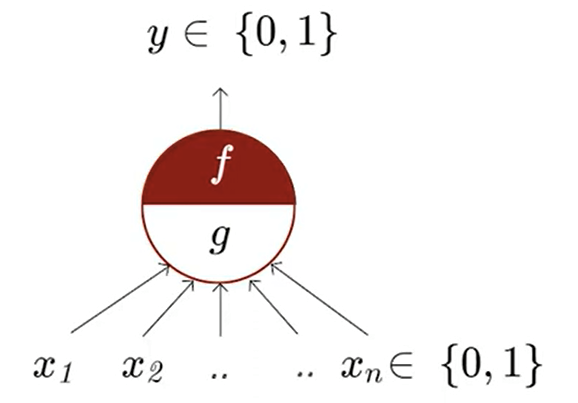
\includegraphics[width=\textwidth]{Degree/static/DL_simple_neuron.png}
             \caption{Simple Model of the Neuron}
             \label{fig:DL-simple-neuron}
         \end{subfigure}
         \hfill
        \begin{subfigure}[b]{0.45\textwidth}
            \centering
            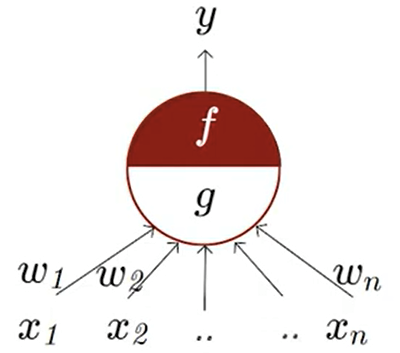
\includegraphics[width=0.71\textwidth]{Degree/static/DL_perceptron.png}
            \caption{Model of the Perceptron}
            \label{fig:DL-perceptron}
        \end{subfigure}
        \caption{First models of neurons}
        \label{fig:DL-first-neurons}
    \end{figure}
\end{itemize}

\subsection{The Deep Revival}
\begin{itemize}
    \item \textbf{Unsupervised Pre-Training}: Described an effective way of initializing the weights that allows deep autoencoders networks to learn a low-dimensional representation of data.
\end{itemize}

\subsection{From Cats to Convolutional Neural Networks}
\begin{itemize}
    \item \textbf{Hubel and Wiesel Experiment}: Experimentally showed that each neuron has a fixed receptive field -i.e. a neuron will fire only in response to visual stimuli in a  specific region in the visual space(Motivation for CNNs).
\end{itemize}

\subsection{Faster, higher, stronger}
\begin{itemize}
    \item \textbf{Better Optimization Methods}: Faster convergence, better accuracies. Examples: AdaGrad, RMSProp, Adam, Nadam, etc.
    \item \textbf{Better Activation Functions}: Many new functions have been proposed, leading to better convergence and performance. Example: tanh, ReLu, Leaky Relu, etc.
\end{itemize}

\subsection{The Curios Case of Sequences}
\begin{itemize}
    \item \textbf{Sequences}: Each unit in the sequence interacts with other units. Need models to capture this interaction. Example: Speech, Videos, etc.
    \item \textbf{Hopfield Network}: Content-addressable memory systems for storing and retrieving patterns.
    \item \textbf{Jordan Network}: The output state of each time step is fed to the next time step, thereby allowing interactions between time steps in the sequence.
    \item \textbf{Elman Network}: The hidden state of each time step is fed to the next time step, thereby allowing interactions between time steps in the sequence.
    \item Very hard to train RNNs.
    \item \textbf{Long Short Term Memory}: Solve complex long time lag tasks that could never be solved before(solved the problem of vanishing gradient).
    \item \textbf{Sequence to Sequence Models}: Introduction to Attention!!, However, they were unable to capture the contextual information of a sentence.
    \item \textbf{Transformers}: Introduced a paradigm shift in the field of NLP. GPT and BERT are the most commonly used transformer based architectures.
\end{itemize}

\subsection{Beating humans at their own game}
\begin{itemize}
    \item Human-level control through deep reinforcement learning for playing Atari Game
    \item \textbf{OpenAI Gym}: Toolkit for developing and comprising reinforcement learning algorithms. It supports teaching agents everything from walking to playing games like Pong or Pinball.
    \item \textbf{OpenAI Gym Retro}: A platform for reinforcement learning research on games, which contains 1,000 games across a variety of backing emulators.
    \item \textbf{MuZero}: Masters Go, chess, shogi and Atari without needing to be told the rules, thanks to its ability to plan winning strategies in unknown environments.
    \item \textbf{Player of Games(PoG)}: A general purpose algorithm that unifies all previous approached. Learn to play under both perfect and imperfect information games.
\end{itemize}

\subsection{The rise of Transformers}
\begin{itemize}
    \item \textbf{Rule Based Systems}: Initial Machine Translation Systems used handcrafted rules and dictionaries to translate sentences between few politically important language pairs.
    \item \textbf{Statistical MT}: The IBM Models for Machine Translation gave a boost to the idea of data driven statistical NLP, probability based models.
    \item \textbf{Neural MT}: The introduction of seq2seq models and attention. Bigger, hungrier, better models.
    \item \textbf{From Language to Vision}: A vision model based as closely as possible on the Transformer architecture, originally designed for text-based tasks.
    \item \textbf{From Discrimination to Generation}: Sample(Generate) data from the learned probability distribution.Variable Auto Encoders(VAE), Generational Adversarial Networks(GAN), Flow-based models to achieve it.
    \item GANs don't scale, are unstable and capture less diversity. Diffusion models are one of the alternatives to GAN. Inspired by an idea from non-equilibrium thermodynamics.
\end{itemize}

\subsection{Call for Sanity}
\begin{itemize}
    \item \textbf{Paradox of Deep Learning}: Deep learning works so well despite high capacity(susceptible to overfitting), numerical instability(vanishing/exploding gradients), sharp minima(leads to overfitting), non-robustness.
    \item \textbf{Interpretable Machine Learning: A Guide for Making Black Box Models Explainable} by Christoph Molnar.
    \item \textbf{AI Audit challenge}: AI systems must be evaluated for legal compliance, in particular laws protecting people from illegal discrimination. This challenge seeks to broaden the tools available to people who want to analyze and regulate them.
    \item \textbf{Analog AI}: Programmable resistors are the key building blocks in analog deep learning, just like transistors are the core element of digital processors(faster computation).
\end{itemize}

\subsection{The AI revolution in basic Science Research}
\begin{itemize}
    \item \textbf{Protein-Folding Problem}: Model proposed to predict protein structure, which would lead to better drug development.
    \item \textbf{Astronomy: Galaxy Evolution}: Predict how galaxies would look like as it gets older.
\end{itemize}

\subsection{Efficient Deep Learning}

\begin{itemize}
    \item Build models on small devices, aka phones. Deploying models in resource-constrained devices.
\end{itemize}

\section{Multi Layered Network of Perceptrons}
\subsection{Biological Neurons}
\begin{itemize}
    \item The most fundamental unit of a deep neural network is called an artificial neuron.
    \item The inspiration comes from biology(more specifically, from the brain).
    \item \textbf{biological neurons = neural cells = neural processing units}
    \item \textbf{Dendrite}: Receives signals from other neurons\\
    \textbf{Synapse}: Point of connection to other neurons\\
    \textbf{Soma}: Processes the information\\
    \textbf{Axon}: Transmits the output of this neuron.
    \item This massively parallel network also ensures that there is division of work. Each neuron may perform a certain role or respond to a certain stimulus. The neurons in the brain arranged in a hierarchy.
    \begin{figure}[H]
        \centering
        \begin{subfigure}[b]{0.3\textwidth}
            \centering
            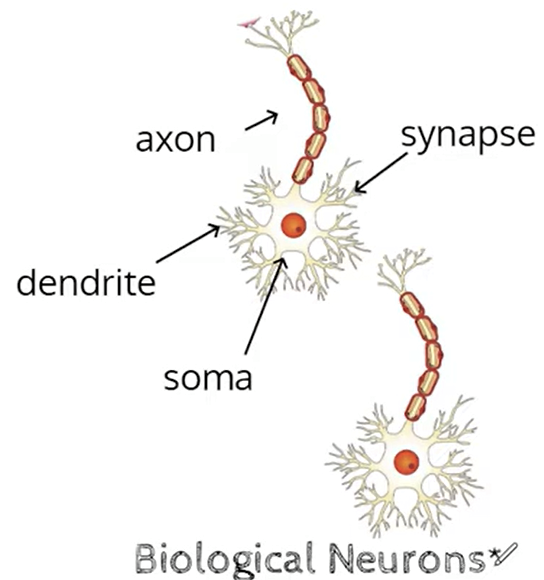
\includegraphics[width=0.9\textwidth]{Degree/static/DL_biological_neuron.png}
            \caption{Biological Neuron}
            \label{fig:DL-biological-neuron}
        \end{subfigure}
        \begin{subfigure}[b]{0.3\textwidth}
            \centering
            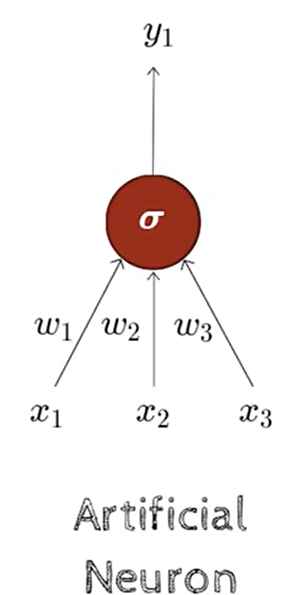
\includegraphics[width=0.5\textwidth]{Degree/static/DL_artificial_neuron.png}
            \caption{Artificial Neuron}
            \label{fig:DL-artificial-neuron}
        \end{subfigure}
        \begin{subfigure}[b]{0.3\textwidth}
            \centering
            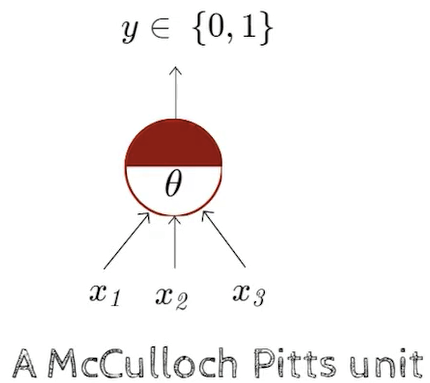
\includegraphics[width=\textwidth]{Degree/static/DL_Pitts_unit.png}
            \caption{A McCulloch Pitts Unit}
            \label{fig:DL-pitts-neuron}
        \end{subfigure}
        \caption{Basic Neuron Structure}
        \label{fig:DL-basic-neurons}
    \end{figure}
    \item \textbf{McCulloch Pitts Neuron}: Proposed a highly simplified computational model of the neuron. $g$ aggregates the inputs, and the function $f$ takes a decision based on this aggregation. The inputs can be excitatory or inhibitory.\\
    \textbf{Example}: $y=0$ if any $x_i$ is inhibitory, else $g(x_1,...,x_n)=g(x)=\sum_{i=1}^nx_i$\\
    $y=f(g(x))=1$ if $g(x)\geq \theta$ else $0$\\
    $\theta$ is called the thresholding parameter.
    \item circle at the end indicates inhibitory input if any inhibitory input is $1$ then the output will be $0$.
    \item Linear separability(for boolean functions): There exists a line(plane) such that all inputs which produce a $1$ lie on one side of the line(plane) and all inputs which produce a $0$ lie on the other side of the line(plane).
    \item A single McCulloch Pitts Neuron can be used to represent boolean functions which are linearly separable.
    \item It can be trivially seen that $\theta=0$ for the Tautology(always ON) function.
    \begin{figure}[H]
        \centering
        \begin{subfigure}[b]{0.225\textwidth}
            \centering
            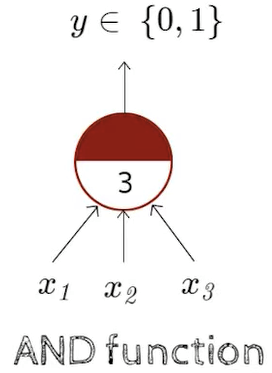
\includegraphics[width=1\textwidth]{Degree//static/DL_Pitts_AND.png}
            \caption{AND function}
            \label{fig:DL-pitts-AND}
        \end{subfigure}
        \hfill
        \begin{subfigure}[b]{0.225\textwidth}
            \centering
            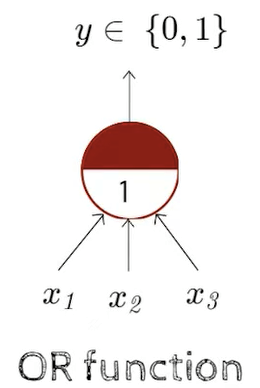
\includegraphics[width=0.9\textwidth]{Degree//static/DL_Pitts_OR.png}
            \caption{OR function}
            \label{fig:DL-pitts-OR}
        \end{subfigure}
        \hfill
        \begin{subfigure}[b]{0.225\textwidth}
            \centering
            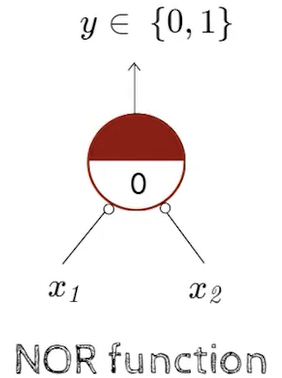
\includegraphics[width=1\textwidth]{Degree//static/DL_Pitts_NOR.png}
            \caption{NOR function}
            \label{fig:DL-pitts-NOR}
        \end{subfigure}
        \hfill
        \begin{subfigure}[b]{0.225\textwidth}
            \centering
            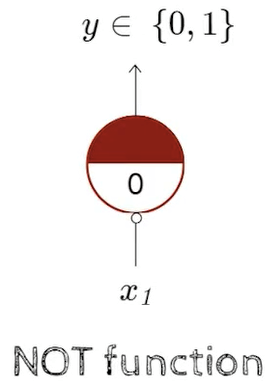
\includegraphics[width=1\textwidth]{Degree//static/DL_Pitts_NOT.png}
            \caption{NOT function}
            \label{fig:DL-pitts-NOT}
        \end{subfigure}
        \caption{Basic Boolean functions}
        \label{fig:DL-basic-boolean}
    \end{figure}
\end{itemize}

\subsection{Perceptrons}
\begin{itemize}
    \item \textbf{Classical Perceptron}: Frank Rosenblatt proposed this model, which was refined and carefully analyzed by Minsky and Papert.
    \item Main difference is the introduction of numerical weights for inputs and a mechanism for learning these weights.
    \item $y=1$ \textit{if} $\sum_{i=1}^nw_i\times x_i \geq \theta$ else $0$.\\
    If we take $\theta$ on one side and represent $w_0=-\theta$ and $x_0=1$, then we have\\
    $y=1$ \textit{if} $\sum_{i=0}^nw_i\times x_i\geq 0$ else $0$.
    \item $w_0$ is called the bias as it represents the \textbf{prior}(prejudice).
    \item From the equation, it can be clearly seen that a perceptron separates the input space into two halves. A single perceptron can only be used to implement linearly separable functions.
    \item The difference between this and the MP neuron is that now we have weights that can be learned, and the inputs can be real values.
    \begin{figure}[H]
        \centering
        \begin{subfigure}[b]{0.45\textwidth}
            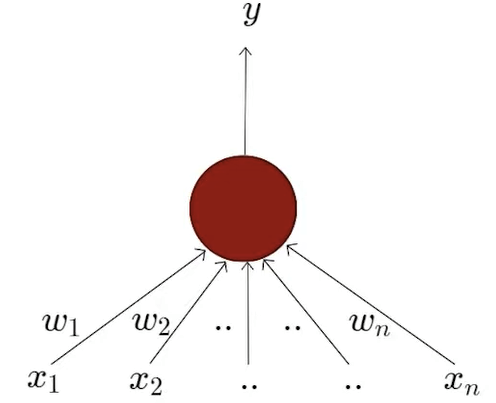
\includegraphics[width=0.8\textwidth]{Degree//static/DL_classical_perceptron.png}
            \caption{Perceptron}
            \label{fig:DL-perceptron-1}
        \end{subfigure}
        \hfill
        \begin{subfigure}[b]{0.45\textwidth}
            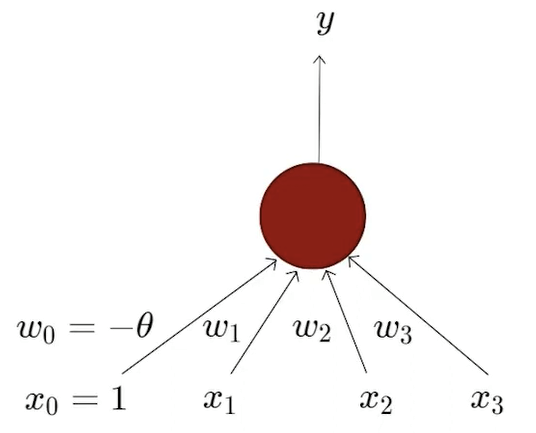
\includegraphics[width=0.8\textwidth]{Degree/static/DL_perceptron_bias.png}
            \caption{Perceptron with $w_0$}
            \label{fig:DL-perceptron-bias}
        \end{subfigure}
        \caption{Classical Perceptrons}
        \label{fig:DL-classical-perceptrons}
    \end{figure}
\end{itemize}

\subsection{Perceptron Learning Algorithm}
\begin{itemize}
    \item \textbf{Perceptron learning algorithm}: Consider two vectors $w=[w_0,...,w_n]$ and $x=[1,x_1,...,x_n]$, then $w\times x=w^Tx$ or the dot product. We can rewrite the perceptron rule as $y=1$ \textit{if} $w^Tx\geq 0$ else $0$.\\
    \item We are interested in finding the line $w^Tx=0$ which divides the input space into two halves. The angle $\alpha$ between $w$ and any point $x$ which lies on the line must be $90^{\circ}$ because $\cos{\alpha}=\frac{w^Tx}{||w||||x||}=0$. So, the vector $w$ is perpendicular to every point on the line, then it is perpendicular to the line itself.
    \item For any point such that $w^Tx>0$ we will have $\alpha<90^{\circ}$ and for any point such that $w^Tx<0$ we will have $\alpha>90^{\circ}$.
    \begin{algorithm}[H]
        \caption{Perceptron Learning Algorithm}\label{alg:DL-perceptron-learning-alg}
        \begin{algorithmic}[1]
            \State $P\gets$ \textit{inputs with label }$1$;
            \State $N\gets$ \textit{inputs with label }$0$;
            \State Initialize \textbf{w} randomly
            \While{!\textit{convergence}}
                \State Pick random $x\in P\cup N$;
                \If{$x\in P$ \textit{and} $\sum_{i=0}^nw_i\times x_i<0$}
                    \State \textbf{w} = \textbf{w} + \textbf{x};
                \EndIf
                \If{$x\in N$ \textit{and} $\sum_{i=0}^nw_i\times x_i\geq 0$}
                    \State \textbf{w} = \textbf{w} - \textbf{x};
                \EndIf
            \EndWhile
            \LComment{the algorithm converges when all the inputs are classified correctly}
        \end{algorithmic}
    \end{algorithm}
    \item For $x\in P$ if $w^Tx<0$ then it means that the angle $\alpha$ between this $x$ and the current $w$ is greater than $90^{\circ}$, but we want it to be $<90^{\circ}$.\\
    When we do $w_{new}=w+x$, alpha changes as follows
    \begin{equation*}
        \cos{\alpha_{new}}\propto (w_{new}^Tx)=(w+x)^Tx=W^Tx+x^Tx=\cos{\alpha}+x^Tx
    \end{equation*}
    \begin{equation*}
        \cos{\alpha_{new}}>\cos{\alpha}\implies \alpha_{new}<\alpha
    \end{equation*}
    $\alpha_{new}$ becomes less than, $\alpha$ which is exactly what we wanted, we may not get $<90^{\circ}$ in one shot so we keep doing it. Similarly, it can be shown for $x\in N$.
    \item \textbf{Definition}: Two sets $P$ and $N$ of points in an $n-$dimensional space are called absolutely linearly separable if $n+1$ real numbers $w_0,...,w_n$ exist such that every point $(x_1,...,x_n)\in P$ satisfies $\sum_{i=1}^nw_i\times x_i\geq w_0$ and every point $(x_1,...,x_n)\in N$ satisfies $\sum_{i=1}^nw_i\times x_i<w_0$.
    \item \textbf{Proposition}: If the sets $P$ and $N$ are finite and linearly separable, the perceptron learning algorithm updates the weight vector $w$ a finite number of times. In other words: if the vectors in $P$ and $N$ are tested cyclically one after the other, a weight vector $w$ is found after a finite number of steps $t$ which can separate the two sets.
    \item \textbf{Proof of Convergence}: If $x\in N$, then $-x\in P$ ($\therefore w^Tx<0\implies w^T(-x)\geq 0$).\\
    We can now consider only a single set $P'=P\cup N^-$ and for every element $p\in P'$ ensure that $w^Tp\geq 0$.
    \begin{algorithm}[H]
        \caption{Modified Perceptron Learning Algorithm}\label{alg:DL-modified-perceptron-learning-alg}
        \begin{algorithmic}[1]
            \State $P\gets$ \textit{inputs with label }$1$;
            \State $N\gets$ \textit{inputs with label }$0$;
            \State $N^-\gets$ \textit{negations of all points in }$N$;
            \State $P'\gets P\cup N^-$
            \State Initialize \textbf{w} randomly
            \While{!\textit{convergence}}
                \State Pick random $p\in P'$;
                \If{$\sum_{i=0}^nw_i\times p_i<0$}
                    \State \textbf{w} = \textbf{w} + \textbf{p};
                \EndIf
            \EndWhile
            \LComment{the algorithm converges when all the inputs are classified correctly}
        \end{algorithmic}
    \end{algorithm}
    Further we will normalize all the $p$'s so that $||p||=1$, notice this does not change anything in our step.\\
    Let $w^*$ be the normalized solution vector(we know one exists whose value we don't know).\\
    Now suppose at some time step $t$ we inspected the point $p_i$ and found that $w^Tp_i<0$, then we make correction $w_{t+1}=w_t+p_i$.\\
    Let $\beta$ be the angle between $w^*$ abd $w_{t+1}$, then we have $\cos{\beta}=\frac{w^*w_{t+1}}{||w_{t+1}||}$
    \begin{equation*}
    \begin{split}
        Numerator\text{ }=w^*\cdot w_{t+1}=x^*\cdot (w_t+p_i)=w^*\cdot w_{t} + w^*\cdot p_i\geq w^*\cdot w_{t}+\delta \text{ }(\delta=\min(w^*\cdot p_i|\forall i))\\
        \geq w^*\cdot(w_{t-1}+p_j)+\delta \geq w^*\cdot w_{t-1} + w^*\cdot p_j + \delta \geq w^*\cdot w_{t-1}+2\delta \geq w^*w_0+(k)\delta \text{ }(By\text{ }Induction)
    \end{split}
    \end{equation*}
    \begin{equation*}
    \begin{split}
        Denominator^2\text{ }=||w_{t+1}||^2=(w_{t}+p_i)\cdot(w_{t}+p_i)=||w_t||^2+2w_t\cdot p_i+||p_i||^2\leq ||w_t||^2+||p_i||^2\\
        \leq ||w_t||^2+1\leq (||w_{t-1}||^2+1)+1\leq ||w_0||^2+(k)
    \end{split}
    \end{equation*}
    So, we have $Numerator\geq w^*\cdot w_0+(k)\delta$ and $Denominator^2\leq ||w_0||^2+(k)$
    \begin{equation*}
        \cos{\beta}\geq \frac{w^*\cdot w_0+k\delta}{\sqrt{||w_0||^2+k}}
    \end{equation*}
    $\cos{\beta}$ grows proportional to $\sqrt{k}$\\
    As $k$(number of corrections) increase $\cos{\beta}$ can become arbitrarily large, but since $\cos{\beta}\leq 1$, $k$ must be bounded by a maximum order.\\
    Thus, there can only be a finite number of corrections $(k)$ to $w$ and the algorithm will converge!
\end{itemize}

\subsection{Linearly Separable Boolean Function}
\begin{itemize}
    \item One simple example that is not linearly separable is XOR
    \begin{table}[H]
        \centering
        \begin{tabular}{cccc}
            \hline
            $x_1$ & $x_2$ & XOR &  \\
            \hline
            0 & 0 & 0 & $w_0+\sum_{i=1}^2w_ix_i<0$\\
            1 & 0 & 1 & $w_0+\sum_{i=1}^2w_ix_i\geq0$\\
            0 & 1 & 1 & $w_0+\sum_{i=1}^2w_ix_i\geq0$\\
            1 & 1 & 0 & $w_0+\sum_{i=1}^2w_ix_i<0$\\
            \hline
        \end{tabular}
        \caption{XOR Truth Table}
        \label{tab:DL-XOR-truth}
    \end{table}
    \item Most real world data is not linearly separable and will always contain some \textbf{outliers}.
    \item How many boolean functions can we design from 2 inputs.
    \begin{table}[H]
        \centering
        \begin{tabular}{cccccccccccccccccc}
            \hline
            $x_1$ & $x_2$ & $f_1$ & $f_2$ & $f_3$ & $f_4$ & $f_5$ & $f_6$ & $f_7$ & $f_8$ & $f_9$ & $f_{10}$ & $f_{11}$ & $f_{12}$ & $f_{13}$ & $f_{14}$ & $f_{15}$ & $f_{16}$ \\
            \hline
            0 & 0 & 0 & 0 & 0 & 0 & 0 & 0 & 0 & 0 & 1 & 1 & 1 & 1 & 1 & 1 & 1 & 1\\
            1 & 0 & 0 & 0 & 0 & 0 & 1 & 1 & 1 & 1 & 0 & 0 & 0 & 0 & 1 & 1 & 1 & 1\\
            0 & 1 & 0 & 0 & 1 & 1 & 0 & 0 & 1 & 1 & 0 & 0 & 1 & 1 & 0 & 0 & 1 & 1\\
            1 & 1 & 0 & 1 & 0 & 1 & 0 & 1 & 0 & 1 & 0 & 1 & 0 & 1 & 0 & 1 & 0 & 1\\
            \hline
        \end{tabular}
        \caption{Functions of 2 inputs}
        \label{tab:DL-2-ip-functions}
    \end{table}
    Out of these, only XOR and !XOR are not linearly separable.
    \item In general, we can have $2^{2^n}$ boolean functions in $n$ inputs.
\end{itemize}

\subsection{Representation Power of a Network of Perceptrons}
\begin{itemize}
    \item We will assume True $=+1$ and False $=-1$, we consider 2 inputs and 4 perceptrons with specific weights. The bias of each perceptron is $-2$. Each of these perceptrons is connected to an output perceptron by weights (which need to be learned). The output of this perceptron $(y)$ is the output of this network.
    \begin{figure}[H]
        \centering
        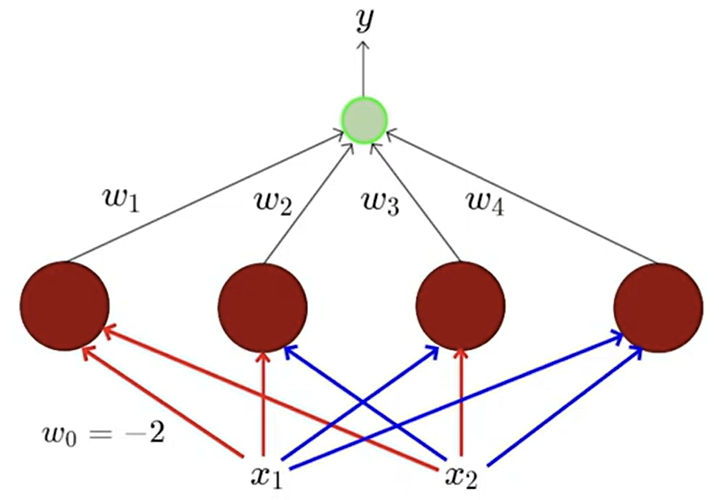
\includegraphics[width=0.5\linewidth]{Degree//static/DL_simple_network.png}
        \caption{Network of Perceptrons}
        \label{fig:DL-simple-network}
    \end{figure}
    red edge indicates $w=-1$, and blue edge indicates $w=+1$. $x_1$ has weights $-1,-1,+1,+1$ and $x_2$ has weights $-1, +1, -1, +1$ from left to right respectively.
    \item The above network contains $3$ layers.\\
    The layer containing the inputs $(x_1,x_2)$ is called the \textbf{input layer}.\\
    The middle layer containing the $4$ perceptrons is called the \textbf{hidden layer}.\\
    The final layer containing one output neuron is called the \textbf{output layer}.\\
    The output of the $4$ perceptrons in the hidden layer are denoted by $h_1,h_2,h_3,h_4$.\\
    The red and blue edges are called layer 1 weights\\
    $w_1,w_2,w_3,w_4$ are called layer 2 weights.
    \item This network can be used to implement \textbf{any} boolean function linearly separable or not. Each perceptron in the middle layer fires only for a specific input and no perceptrons fire for the same input.
    \begin{table}[H]
        \centering
        \begin{tabular}{cccccccc}
            \hline
            $x_1$ & $x_2$ & XOR &  $h_1$ & $h_2$ & $h_3$ & $h_4$ & $\sum_{i=1}^4w_ih_i $\\
            \hline
            0 & 0 & 0 & 1 & 0 & 0 & 0 & $w_1$\\
            1 & 0 & 1 & 0 & 1 & 0 & 0 & $w_2$\\
            0 & 1 & 1 & 0 & 0 & 1 & 0 & $w_3$\\
            1 & 1 & 0 & 0 & 0 & 0 & 1 & $w_4$\\
            \hline
        \end{tabular}
        \caption{Truth Table for the Network}
        \label{tab:DL-network-truth}
    \end{table}
    This results in four independent conditions.
    \item In case of $3$ inputs we would now have $8$ perceptrons in the hidden layer.
    \item \textbf{Theorem}: Any boolean function of $n$ inputs can be represented exactly by a network of perceptrons containing one hidden layer with $2^n$ perceptrons and one output layer containing 1 perceptron.
    \item \textbf{Note}: A network of $2^n+1$ perceptrons is not necessary but sufficient.
    \item \textbf{Catch}: As $n$ increases the number of perceptrons in the hidden layers increases exponentially.
    \item We care about boolean functions, because we can model real world examples into boolean functions or classification problems.
    \item The network we saw is formally known as Multilayer Perceptron(MLP) or more appropriately "Multilayered Network of Perceptrons".
\end{itemize}

\section{Sigmoid Neurons}

\subsection{What are they?}
\begin{itemize}
    \item The thresholding logic used by a perceptron is very harsh! It is a characteristic of the perceptron function itself which behaves like a \textbf{step function}.
    \item For most real world applications we would expect a smoother decision function which gradually changes from 0 to 1.
    \item Instead we would use sigmoid function
    \begin{equation*}
        y=\frac{1}{1+\exp(-(\omega_0+\sum_{i=1}^n\omega_ix_i))}
    \end{equation*}
    \item We no longer see a sharp transition around the threshold $\omega_0$. Also, $y$ now takes any real value in $[0,1]$.
    \item This value can also be interpreted as probability.
\end{itemize}

\subsection{Typical Supervised Machine Learning Setup}\label{sec:DL-typical-ml-setup}
\begin{itemize}
    \item \textbf{Data}: $\{x_i,y_i\}_{i=1}^n$, we have $n$ data point where $x_i$ is a vector of $\mathbb{R}^m$. Assume $y=\hat{f}(x;\theta)$.
    \item \textbf{Model}: Our approximation of the relation between $x$ and $y$.
    \begin{equation*}
        \text{For example, }\hat{y}=\frac{1}{1+e^{-w^Tx}}\text{ or }\hat{y}=w^Tx\text{ or }\hat{y}=x^TWx
    \end{equation*}
    \item \textbf{Learning algorithm}: An algorithm for learning the parameters $w$ of the model.
    \item \textbf{Objective/Loss/Error function}: To guide the learning algorithm. One possibility is $\sum_{i=1}^n(\hat{y}_i-y_i)^2$.
    \item The learning algorithm should aim to minimize the loss function.
\end{itemize}

\subsection{Learning Parameters}
\begin{itemize}
    \item For ease of explanation we will take $f(x)=\frac{1}{1+e^{-(wx+b)}}$, only a single parameter.
    \item Assume input for training data is $\{x_i,y_i\}_{i=1}^N\rightarrow$ $N$ pairs of $(x,y)$.
    \item Training Objective: Find $w$ and $b$ such that $\mathcal{L}(w,b)=\frac{1}{N}\sum_{i=1}^N(y_i-f(x_i))^2$ is minimized.
    \item \textbf{Guess Work(Infeasible)}: Intuitively guess what should be the values of $w$ and $b$. May never end and is not feasible for writing algorithms.
    \item \textbf{Update rule}: $\theta_{new}=\theta + \eta \Delta \theta$, how to find $\Delta \theta$?
    \item \textbf{Taylor Series}: A way of approximating any continuously differentiable function $\mathcal{L}(w)$ using polynomials of degree $n$. The higher the degree the better the approximation!
    \begin{equation*}
        \mathcal{L}(w)=\mathcal{L}(w_0)+\frac{\mathcal{L}'(w_0)}{1!}(w-w_0)+\frac{\mathcal{L}''(w_0)}{2!}(w-w_0)^2+...
    \end{equation*}
    \item Linear approximation is the first order approximation of the Taylor series. Quadratic approximation is the second order approximation of the Taylor series.
    \item \textbf{Key point}: You can only do this for a very small $\Delta=w-w_0$.
    \item Let's assume $\Delta \theta=u$, then from Taylor series we have
    \begin{equation*}
        \mathcal{L}(\theta+\eta u)=\mathcal{L}(\theta)+\eta u^T\nabla_\theta \mathcal{L}(\theta)+\frac{\eta^2}{2!}u^T\nabla_\theta^2\mathcal{L}(\theta)u+... = \mathcal{L}(\theta)+\eta u^T\nabla_\theta \mathcal{L}(\theta)
    \end{equation*}
    \item $\eta$ is typically small, so $\eta^2, \eta^3,...\rightarrow 0$
    \item Now, we want new loss less than the current loss
    \begin{equation*}
        \mathcal{L}(\theta+\eta u)-\mathcal{L}(\theta)<0\implies u^T\nabla_\theta \mathcal{L}(\theta)<0
    \end{equation*}
    \item Let $\beta$ be the angle between $u^T$ and $\nabla_\theta \mathcal{L}(\theta)$ and $k=\lVert u^T\rVert \lVert\nabla_\theta \mathcal{L}(\theta)\rVert$, then we can write
    \begin{equation*}
        -1\leq cos(\beta) = \frac{u^T\nabla_\theta \mathcal{L}(\theta)}{\lVert u^T \rVert \lVert \nabla_\theta \mathcal{L}(\theta)\rVert}\leq 1\implies -k\leq u^T\nabla_\theta \mathcal{L}(\theta)\leq k
    \end{equation*}
    \item $u^T\nabla_\theta \mathcal{L}(\theta)$ is most negative when $cos(\beta)=-1$ or $\beta=180^\circ$
    \item \textbf{Parameter Update Rule}: From the above we can now say
    \begin{equation*}
        w_{t+1} = w_t-\eta \nabla w_t
    \end{equation*}
    \begin{equation*}
        b_{t+1} = b_t - \eta \nabla b_t
    \end{equation*}
    \item We can now write the gradient descent algorithm for our problem as follows
    \begin{algorithm}[H]
        \caption{Gradient Descent}\label{alg:SE-Gradient-Descent}
        \begin{algorithmic}[1]
            \Statex \Call{GradientDescent}{}
            \State $t\gets 0$
            \State $max\_iterations \gets$ $1000$
            \State $w,b \gets$ initialize randomly
            \While{$t<$ $max\_iterations$}
                \State $w_{t+1}\gets$ $w_t-\eta \nabla w_t$
                \State $b_{t+1}\gets$ $b_t-\eta \nabla b_t$
                \State $t\gets$ $t+1$
            \EndWhile
        \end{algorithmic}
    \end{algorithm}
    \item where $\nabla w$ and $\nabla b$ are defined for sigmoid neuron as
    \begin{equation*}
        \nabla w=\frac{\partial \mathcal{L}(x)}{\partial w} = (f(x)-y)\frac{\partial}{\partial w}(\frac{1}{1+e^{-(wx+b)}})=(f(x)-y)\times f(x)\times (1-f(x))\times x
    \end{equation*}
    \begin{equation*}
        \nabla b=\frac{\partial \mathcal{L}(x)}{\partial b}=(f(x)-y)\times f(x)\times (1-f(x))
    \end{equation*}
\end{itemize}

\subsection{Representation Power of a multiplayer network of sigmoid neurons}
\begin{itemize}
    \item A multilayer network of neurons with a single hidden layer can be used to approximate any continuous function to any desired precision.
\end{itemize}

\section{Feed Forward Neural Networks}
\subsection{Structure of Feed Forward Neural Network}
\begin{itemize}
    \item The input to the network is an $n-$dimensional vector.
    \item The network contains $L-1$ hidden layers having $n$ neurons each. Value of $n$ could be different in each layer.
    \item Finally, there is one output layer containing $k$ neurons, corresponding to $k classes$.
    \item Each neuron in the hidden layer and output layer can be split into two parts: pre-activation and activation($a_i$ and $h_i$ are vectors).
    \item The input layer can be called the $0-$th layer and the output layer can be called the $L-$th layer.
    \item $W_i\in \mathbb{R}^{n\times n}$ and $b_i\in \mathbb{R}^n$ are the weight and bias between layers $i-1$ and $i$ ($0<i<L$).
    \item $W_L\in \mathbb{R}^{k\times n}$ and $b_L\in \mathbb{R}^k$ are the weight and bias between the last hidden layer and the output layer.
    \item The pre-activation at layer $i$ is given by
    \begin{equation*}
        a_i(x)=b_i+W_ih_{i-1}(x)
    \end{equation*}
    \item The activation at layer $i$ is given by
    \begin{equation*}
        h_i(x)=g(a_i(x))
    \end{equation*}
    \item $g$ is an element wise function and is called the \textbf{activation function}.
    \item The activation at the output layer is given by
    \begin{equation*}
        f(x)=h_L(x)=O(a_L(x))
    \end{equation*}
    where $O$ is the output activation function
    \item For ease of notation $a_i(x)=a_i$ and $h_i(x)=h_i$.
    \item We also have $h_0=x$ and $h_L=\hat{y}=\hat{f}(x)$
    \item We can write $\hat{y}$ as
    \begin{equation*}
        \hat{y}_i=\hat{f}(x_i)=O(W_{3}g(W_{2}g(W_{1}x_i+b_1)+b_2)+b_3)
    \end{equation*}
    This becomes our model as specified in \ref{sec:DL-typical-ml-setup}.
    \item Parameters become $\theta=W_1,...,W_L,b_1,...,b_L$
    \item We can now write our gradient descent algorithm more concisely as
    \begin{algorithm}[H]
        \caption{Gradient Descent Modified}\label{alg:DL-gradien-descent-modified}
        \begin{algorithmic}[1]
            \Statex \Call{Gradient-Descent}{ }
            \State $t\gets$ 0;
            \State $max_iterations\gets$ 1000;
            \State Initialize $\theta_0=[W_1^0,...,W_L^0,b_1^0,....,b_L^0]$
            \While{$t++<$ $max_iterations$}
                \State $\theta_{t+1}\gets$ $\theta_t-\eta \nabla \theta_t$
            \EndWhile
        \end{algorithmic}
    \end{algorithm}
    where we have
    \begin{equation*}
        \theta=[W_1,...,W_L,b_1,....,b_L]\text{ and }\nabla \theta_t=[\frac{\partial \mathcal{L}(\theta)}{\partial W_{1,t}},...,\frac{\partial \mathcal{L}(\theta)}{\partial W_{L,t}},\frac{\partial \mathcal{L}(\theta)}{\partial b_{1t}},...,\frac{\partial \mathcal{L}(\theta)}{\partial b_{1t}}]^T
    \end{equation*}
    \begin{figure}[H]
        \centering
        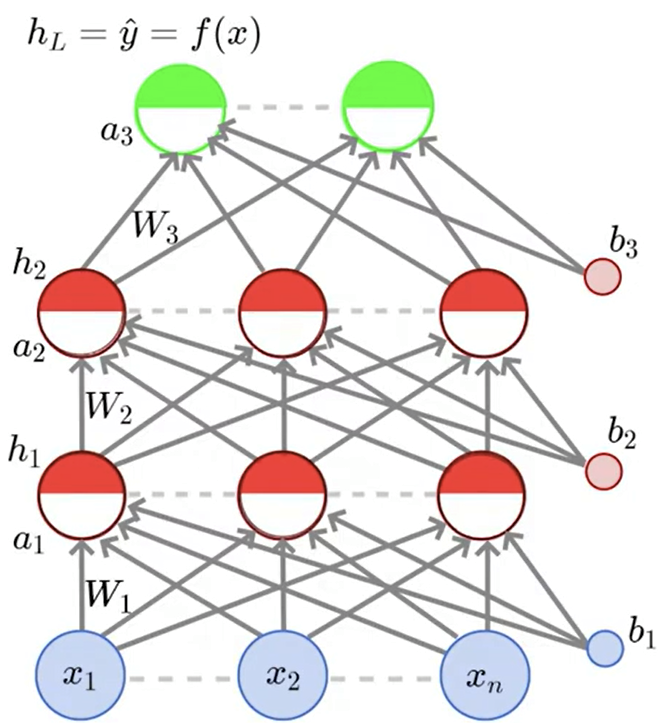
\includegraphics[width=0.5\linewidth]{Degree//static/DL_Feedforward_network.png}
        \caption{Feed Forward Network}
        \label{fig:DL-feedforward-network}
    \end{figure}
\end{itemize}

\subsection{Output functions and Loss functions}
\begin{itemize}
    \item Assume we are trying to predict values in the range of all real values, an appropriate loss function would be mean squared error function.
    \begin{equation*}
        \mathcal{L}(\theta)=\frac{1}{N}\sum_{i=1}^N\sum_{j=1}^k(\hat{y}_{ij}-y_{ij})^2
    \end{equation*}
    \item If we want to predict values in the range of real values, regression, then we can take the output function as a linear function
    \begin{equation*}
        f(x)=h_L=O(a_L)=W_Oa_L+b_O
    \end{equation*}
    \item Given that we are performing classification, then we can use cross entropy loss function. This is known as negative log likelihood function.
    \begin{equation*}
        -\frac{1}{N}\sum_{i=1}^N\sum_{j=1}^k(y_{ij}log(\hat{y}_{ij}) + (1-y_{ij})log(1-\hat{y}_{ij}))
    \end{equation*}
    \item Ensure that $\hat{y}$ is a probability distribution, one appropriate output function can be the softmax function
    \begin{equation*}
        \hat{y}_j=O(a_L)_j=\frac{e^{a_{L,j}}}{\sum_{i=1}^kw^{a_{L,i}}}
    \end{equation*}
    \begin{table}[H]
        \centering
        \begin{tabular}{|c|c|c|}
            \hline
             & Real Values & Probabilities \\
             \hline
            Output Activation & Linear & Softmax\\
            \hline
            Loss Function & Squared Error & Cross Entropy\\
            \hline
        \end{tabular}
        \caption{Choice of Output and Loss functions based on type of Output}
    \end{table}
\end{itemize}
\pagebreak

\subsection{Backpropagation}
\begin{itemize}
    \item Intuitively it can be written as
    \begin{figure}[H]
        \centering
        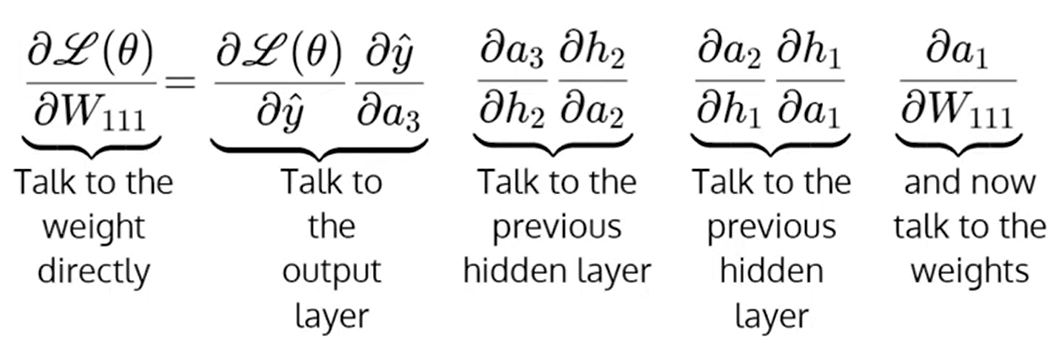
\includegraphics[width=0.5\linewidth]{Degree//static/DL_backprop_intuitie.png}
        \caption{Backpropagation Intuition}
        \label{fig:DL-backprop-intuition}
    \end{figure}
    \item For further discussion, the output function is considered to be softmax and the loss function is considered to be cross entropy.
    \item \textbf{Gradient w.r.t output layer}: We start with the part "Talk to the output layer".
    \begin{equation*}
        \mathcal{L}(\theta) = -\log{\hat{y}_l}\text{ }(l=\text{ true class label})
    \end{equation*}
    \begin{equation*}
        \frac{\partial}{\partial \hat{y}_i}\mathcal{L}(\theta)=\begin{cases}
            -\frac{1}{\hat{y}_l},\text{ if }i=l\\
            0,\text{ otherwise}
        \end{cases}=[0,...,0,-\frac{1}{\hat{y}_l},0,...,0]^T=-\frac{1}{\hat{y}_l}e_l
    \end{equation*}
    $e_l$is a $k-$dimensional vector whose $l^{th}$ element is $1$ and rest are $0$.
    \begin{equation*}
        \frac{\partial \mathcal{L}(\theta)}{\partial a_{L,i}}=-\frac{1}{\hat{y}_l}\frac{\partial \hat{y_l}}{\partial a_{L,i}}
    \end{equation*}
    Since, $\hat{y}_l$ is calculated using cross entropy it is dependent on all $a_L,i$
    \begin{equation*}
        \hat{y}_j=\frac{e^{a_{Lj}}}{\sum_ie^{a_{Li}}}
    \end{equation*}
    \begin{equation*}
        \frac{\partial \hat{y}_l}{\partial a_{L,i}}=\begin{cases}
            \hat{y}_l(1-\hat{y}_l),\text{ if }i= l\\
            -\hat{y}_l\hat{y}_i,\text{ if }i\neq l
        \end{cases}
    \end{equation*}
    We can now write the entire derivative in one shot as
    \begin{equation*}
        \frac{\partial \mathcal{L}(\theta)}{\partial a_{L,i}}=-\frac{1}{\hat{y}_l}(\hat{y}_l)(1_{l=i}-\hat{y}_i)=-(e_l-\hat{y})
    \end{equation*}
    \item \textbf{Chain rule among multiple paths}: If a function $p(z)$ can be written as a function of intermediate results $q_i(z)$ then we have
    \begin{equation*}
        \frac{\partial p(z)}{\partial z}=\sum_m\frac{\partial p(z)}{\partial q_m}\frac{\partial q_m}{\partial z}
    \end{equation*}
    \item \textbf{Gradient w.r.t hidden units}: Now we "Talk to the hidden layers", in this case $p(z)$ is the loss function, $z=h_{ij}$ and $q_m(z)=a_{Lm}$. We have
    \begin{equation*}
        \frac{\partial \mathcal{L}(\theta)}{\partial h_{ij}}=\sum_{m=1}^k\frac{\mathcal{L}(\theta)}{\partial a_{i+1,m}}W_{i+1,m,j}
    \end{equation*}
    \begin{equation*}
        \frac{\partial \mathcal{L}(\theta)}{\partial a_{ij}}=\frac{\partial \mathcal{L}(\theta)}{\partial h_{ij}}\frac{\partial h_{ij}}{\partial a_{ij}}=\frac{\partial \mathcal{L}(\theta)}{\partial h_{ij}}g'(a_{ij})
    \end{equation*}
    \item \textbf{Gradient w.r.t Parameters}: Finally, we "talk to the weights"
    \begin{equation*}
        \frac{\partial \mathcal{L}(\theta)}{\partial W_{kij}}=\frac{\partial \mathcal{L}(\theta)}{\partial a_{ki}}\frac{\partial a_{ki}}{\partial W_{kij}}=\frac{\partial \mathcal{L}(\theta)}{\partial a_{ki}}h^T_{k-1,j}
    \end{equation*}
    \begin{equation*}
        \frac{\partial \mathcal{L}(\theta)}{\partial b_{ki}}=\frac{\partial \mathcal{L}(\theta)}{\partial a_{ki}}\frac{\partial a_{ki}}{\partial b_{ki}}=\frac{\partial \mathcal{L}(\theta)}{\partial a_{ki}}
    \end{equation*}
    \item We can now write the full pseudocode as
    \begin{algorithm}[H]
        \caption{Forward Propagation}\label{alg:DL-forward-pass}
        \begin{algorithmic}[1]
            \For{$k=1$ to $L-1$}
                \State $a_k$ = $b_k+W_kh_{k-1}$
                \State $h_k$ = $g(a_k)$
            \EndFor
            \State $a_L$ = $b_L+W_Lh_{L-1}$
            \State $\hat{y}$ = $O(a_L)$
        \end{algorithmic}
    \end{algorithm}
    \begin{algorithm}[H]
        \caption{Backward Propagation}\label{alg:DL-backward-pass}
        \begin{algorithmic}[1]
            \State $\nabla_{a_L}\mathcal{L}(\theta)=-(e(y)-\hat{y})$
            \For{$k=L-1$ to $1$}
                \State $\nabla_{W_k}\mathcal{L}(\theta)$ = $\nabla_{a_k}\mathcal{L}(\theta)h_{k-1}^T$
                \State $\nabla_{b_k}\mathcal{L}(\theta)$ = $\nabla_{a_k}\mathcal{L}(\theta)$
                \State $\nabla_{h_{k-1}}\mathcal{L}(\theta)=W_k^T\nabla_{a_k}\mathcal{L}(\theta)$
                \State $\nabla_{a_{k-1}}\mathcal{L}(\theta)=\nabla_{h_{k-1}}\mathcal{L}(\theta)\odot [...,g'(a_{k-1,j}),...]$
            \EndFor
        \end{algorithmic}
    \end{algorithm}
    \item $g'$ for logistic function $\sigma(z)$ is $g(z)(1-g(z))$ and for tanh function is $1-(g(z))^2$.
    \item On flat surfaces, gradient descent moves very slow. How do we solve this?
\end{itemize}

\section{Gradient Descent Types}
\subsection{Momentum based Gradient Descent}
\begin{itemize}
    \item \textbf{Intuition}: If I am repeatedly being asked to move in the same direction then I should probably gain some confidence and start taking bigger steps in that direction. Just as a ball gains momentum while rolling down a slope.
    \item Update rule for momentum based gradient descent is
    \begin{equation*}
        \begin{split}
            &u_t=\beta u_{t-1}+\nabla w_t,\hspace{1cm}u_0=\nabla w_0,\text{ }u_{-1}=0\\
            &w_{t+1}=w_t-\eta u_t
        \end{split}
    \end{equation*}
    \item We are not only considering the current gradient, but we are also giving some importance to past history. $\beta$ is typically less than 1, so we give decreasing importance to previous histories. We have
    \begin{equation*}
        u_t = \beta u_{t-1}+\nabla w_t = \beta^2u_{t-2}+\beta \nabla w_{t-1}+\nabla w_t = ... = \sum_{\tau=0}^t\beta^{t-\tau}\nabla w_\tau
    \end{equation*}
    \item In addition to current update, also look at the history of updates.
    \item Even in the regions having gentle slopes, momentum based gradient descent is able to take large steps because the momentum carries it along.
    \item However, there is a possibility of overshooting our goal. This overshoot could lead to oscillations as well.
    \item Despite these oscillations, it will converge faster than gradient descent.
\end{itemize}

\subsection{Nesterov Accelerated Gradient Descent}
\begin{itemize}
    \item Can we do something to reduce the oscillations observed in momentum based gradient descent?
    \item \textbf{Intuition}: Look before you leap, we ask the weights to move by two parts $\beta u_{t-1}$ and $\nabla w_t$. The idea is to first move by $\beta u_{t-1}$ and then compute $\nabla w_t$. So instead of relying only on current gradient we are essentially "looking ahead" and computing new gradient.
    \item Update rule for NAG is
    \begin{equation*}
        \begin{split}
            &u_t = \beta u_{t-1} + \nabla (w_t-\beta u_{t-1})\\
            &w_{t+1} = w_t - \eta u_t\\
            &\text{with }u_{-1}=0,\text{ and }0\leq \beta \leq 1
        \end{split}
    \end{equation*}
\end{itemize}

\subsection{Stochastic vs Batch Gradient Descent}
\begin{itemize}
    \item Regular gradient descent goes over the entire data once before updating the parameters. Because this is the true gradient of the loss as derived earlier. Hence, theoretical guarantees hold.
    \item Imagine we have a million points in the training data, then it will take very long.
    \item In \textbf{stochastic} version, we update the parameters for every point in the data. Now if we have a million data points then we will make a million updates in each epoch.
    \item However, this is an approximate gradient. Hence, we have no guarantee that each step will decrease the loss.
    \item So, going over a large data once is bad, going over a single point and updating is bad, but going over some data points and updating is ok.
    \item This is the idea for \textbf{mini-batch} gradient descent.
    \item 1 epoch is one pass over the entire data, 1 step is one update of the parameters, $N$ is the number of data points, and $B$ is the mini batch size.
    \item So, for regular gradient descent the number of epochs is the same as number of steps, for stochastic gradient descent the number of steps is the same as $N$, and for mini-batch gradient descent the number of steps is the same as $\frac{N}{B}$.
    \item It is intuitive that a larger batch size is better, but we sacrifice on time.
    \begin{table}[H]
        \centering
        \begin{tabular}{|c|c|}
            \hline
            \textbf{Algorithm} & \textbf{\# of steps in 1 epoch}\\
            \hline
            Vanilla (Batch) Gradient Descent & 1 \\
            \hline
            Stochastic Gradient Descent & $N$\\
            \hline
            Mini Batch Gradient Descent & $\frac{N}{B}$\\
            \hline
        \end{tabular}
        \caption{Stochastic vs Mini Batch Gradient Descent}
        \label{tab:DL-stochastic-vs-mini-batch}
    \end{table}
\end{itemize}

\subsection{Scheduling Learning Rate}
\begin{itemize}
    \item Instead of using momentum and NAG we could have simply increased the learning rate, but on regions which have a steep slope, the already large gradient would blow up farther.
    \item What we need is for the learning rate to be small when gradient is high and vice versa.
    \item Tune learning rate, try different values on a log scale: $0.0001, 0.001, 0.001, 0.1, 1.0$.
    \item Run a few epochs with each of these and figure out a learning rate which works best. Now do a finer search around this value.
    \item These are just heuristics, no clear winning strategy.
    \item \textbf{Annealing learning rate}: Decrease the learning rate as we get close to the minima.
    \item \textbf{Step Decay}: Halve the learning rate after every 5 epochs or halve the learning rate after an epoch if the validation error is more than what it was at the end of the previous epoch.
    \item \textbf{Exponential Decay}: $\eta = \eta_0^{-kt}$, where $\eta_0$ and $k$ are hyperparameters and $t$ is a step number. However, choosing $k$ becomes complex.
    \item \textbf{1/t Decay}: $\eta = \frac{\eta_0}{1+kt}$, again choosing $k$ is a bit tricky, ideally we won't use these learning rates.
    \item For momentum the following schedule was suggested by Sutskever et al., 2013
    \begin{equation*}
        \beta_t = min(1-2^{-1-\log_2{(\lfloor \frac{t}{250}\rfloor+1})},\beta_{max})
    \end{equation*}
    $\beta_{max}$ is chosen from $\{0.999,0.995,0.99,0.9,0\}$
    \item In practice, often a line search is done to find a relatively better value of $\eta$. Update $w$ using different values of $\eta$ then pick the best $w$ based on loss function.
\end{itemize}

\section{Adaptive Learning Rates}
\begin{itemize}
    \item \textbf{Intuition}: Decay the learning rate for parameters in proportion to their update history(more updates means more decay).
    \item Update rule for \textbf{AdaGrad}
    \begin{equation*}
        \begin{split}
            &v_t = v_{t-1} + (\nabla w_t)^2\\
            &w_{t+1} = w_t - \frac{\eta}{\sqrt{v_t+\epsilon}}\times \nabla w_t
        \end{split}
    \end{equation*}
    and similar set of equations for $b_t$.
    \item \textbf{Intuition}: AdaGrad decays the learning rate very aggressively(as the denominator grows). As a result, after a while, the frequent parameters will start receiving very small updates. To avoid this we can decay the denominator.
    \item Update rule for \textbf{RMSprop}
    \begin{equation*}
        \begin{split}
            &v_t = \beta v_{t-1} + (1-\beta)(\nabla w_t)^2\\
            &w_{t+1}=w_t-\frac{\eta}{\sqrt{v_t+\epsilon}}\times \nabla w_t
        \end{split}
    \end{equation*}
    Give lower and lower weightage to previous gradients
    \item RMSprop converges more quickly than AdaGrad by being less aggressive on decay.
    \item In RMSprop, the deltas start oscillating after a while, learning rate can increase, decrease or remain constant. Whereas in AdaGrad learning rate can only decrease as the denominator constantly grows.
    \item In case of oscillations, setting $\eta_0$ properly could solve the problem.
    \item Both are \textbf{sensitive} to initial learning rate, initial conditions of parameters and corresponding gradients.
    \item \textbf{AdaDelta} avoids setting initial learning rate $\eta_0$
    \begin{equation*}
        \begin{split}
            &v_t = \beta v_{t-1} + (1-\beta)(\nabla w_t)^2\\
            &\Delta w_t = -\frac{\sqrt{u_{t-1}+\epsilon}}{\sqrt{v_t+\epsilon}}\nabla w_t\\
            &w_{t+1} = w_t+\Delta w_t\\
            &u_t = \beta u_{t-1}+(1-\beta)(\Delta w_t)^2
        \end{split}
    \end{equation*}
    Now the numerator, in the effective learning rate, is a function of past gradients. Observe that the $u_t$ that we compute at $t$ will be used only in the next iteration. Essentially one history runs behind the other.
    \item After some $i$ iterations, $v_t$ will start decreasing and the ratio of the numerator to the denominator starts increasing. If the gradient remains low for a subsequent time steps, then the learning rate grows accordingly.
    \item Therefore, AdaDelta allows the numerator to increase or decrease based on the current and past gradients.
    \item \textbf{Intuition}: Do everything that RMSprop does to solve the decay problem of AdaGrad, plus used a cumulative history of the gradients.
    \item Update rule for \textbf{Adam(Adaptive Moments)}
    \begin{equation*}
        \begin{split}
            &m_t = \beta_1m_{t-1}+(1-\beta_1)\nabla w, \text{   }\hat{m}_t = \frac{m_t}{1-\beta_1^t}\gets \text{Incorporating classical momentum}\\
            &v_t = \beta_2v_{t-1}+(1-\beta_2)(\nabla w_t)^2, \text{   }\hat{v}_t = \frac{v_t}{1-\beta_2^t}\\
            &w_{t+1} = w_t - \frac{\eta}{\sqrt{\hat{v}_t}+\epsilon}\hat{m}_t
        \end{split}
    \end{equation*}
    Note that we are taking a running average of the gradients as $m_t$.
    \item One way of looking at this is that we are interested in the expected value of the gradient and not on a single point estimate computed at time $t$.
    \item $\hat{m}_t$ and $\hat{v}_t$ are bias correction terms, we do this to avoid very high learning rate update. It can also be derived by taking expectation of $m_t$.
    \item Bias correction is the problem of exponential averaging.
    \item General form of $L^p$ norm is $(|x_1|^p+|x_2|^p+...+|x_n|^p)^{\frac{1}{p}}$, as $p\to \infty$, $L^p$ boils down to taking the max value.
    \item In Adam, we called $\sqrt{v_t}$ as $L^2$ norm, why not replace it with $L^{\infty}$ norm. Therefore, we have
    \begin{equation*}
        \begin{split}
            &v_t = \max(\beta_2^{t-1}|\nabla w_1|, \beta_2^{t-2}|\nabla w_2|, ..., |\nabla w_t|)\\
            &v_t = \max(\beta_2v_{t-1}, |\nabla w_t|)\\
            &w_{t+1} = w_t-\frac{\eta_0}{v_t}\nabla w_t
        \end{split}
    \end{equation*}
    Observe that we didn't use bias corrected $v_t$ as max norm is not susceptible to initial zero bias.
    \item Suppose that we initialize $w_0$ such that the gradient at the $w_0$ is high. Suppose further that the gradients for the next subsequent iterations are also zero because $x$ is sparse. Ideally, we don't want the learning rate to change its value when $\nabla w_t=0$.
    \item Update Rule for \textbf{MaxProp} is similar to RMSprop
    \begin{equation*}
        \begin{split}
            &v_t = \max(\beta v_{t-1}, |\nabla w_t|)\\
            &w_{t+1} = w_t - \frac{\eta}{v_t+\epsilon}\nabla w_t
        \end{split}
    \end{equation*}
    \item We can extend the same idea to Adam and call it \textbf{AdaMax}
    \begin{equation*}
        \begin{split}
            &m_t = \beta_1m_{t-1} + (1-\beta_1)\nabla e_t,\text{   }\hat{m}_6 = \frac{m_t}{1-\beta_1^t}\\
            &v_t = \max(\beta_2v_{t-1}, |\nabla w_t|)\\
            &w_{t+1} = w_t-\frac{\eta}{v_t+\epsilon}\hat{m}_t
        \end{split}
    \end{equation*}
    \item \textbf{Intuition}: We know NAG is better than momentum based GD, why not just incorporate it with Adam.
    \item We can rewrite NAG such that there is no $t-1$ term, as
    \begin{equation*}
        \begin{split}
            &g_{t+1} = \nabla w_t\\
            &m_{t+1} = \beta m_t + \eta g_{t+1}\\
            &w_{t+1} = w_t - \eta(\beta m_{t+1} + g_{t+1})
        \end{split}
    \end{equation*}
    \item Update rule for \textbf{NAdam(Nesterov Adam)}
    \begin{equation*}
        \begin{split}
            &m_t = \beta_1m_{t-1}+(1-\beta_1)\nabla w, \text{   }\hat{m}_t = \frac{m_t}{1-\beta_1^t}\\
            &v_t = \beta_2v_{t-1}+(1-\beta_2)(\nabla w_t)^2, \text{   }\hat{v}_t = \frac{v_t}{1-\beta_2^t}\\
            &w_{t+1} = w_t - \frac{\eta}{\sqrt{\hat{v}_{t+1}}+\epsilon}(\hat{m}_{t+1}+\frac{(1-\beta_1)\nabla w_t}{1 - \beta_1^{t+1}})
        \end{split}
    \end{equation*}
    \item It is common for new learners to start out using off the shelf optimizers, which are later replaced by custom designed ones.
    \item \textbf{Cyclical Learning Rate}: Suppose the loss surface has a saddle point. Suppose further that the parameters are initialized, and the learning rate is decreased exponentially. After some iterations, the parameters will reach near the saddle point. Since, the learning rate has decreased exponentially, the algorithm has no way of coming out of the saddle point.\\
    What if we allow the learning rate to increase after some iterations.
    \item \textbf{Rationale}: Often, difficulty in minimizing the loss arises from saddle points rather than poor local minima.
    \item A simple way to solve this is to vary the learning rate cyclically. One example is triangular learning rate.
    \item \textbf{Cosine Annealing(Warm Re-Start)}: also based on cyclical learning rate
    \begin{equation*}
        \eta_t = \eta_{min} + \frac{\eta_{max}-\eta_{min}}{2}(1+\cos(\pi \frac{t\%(T+1)}{T})), \text{ }T\text{ is restart interval}
    \end{equation*}
    \item \textbf{Warm-start}: Using a low initial learning rate helps the model to warm and converge better.
\end{itemize}

\section{Regularization}
\subsection{Introduction to Bias and Variance}
\begin{itemize}
    \item Deep learning models typically have BILLIONS of parameters whereas the training data may have only MILLIONS of samples. Therefore, they are called \textbf{over-parameterized} models.
    \item Over-parameterized models are \textbf{prone} to a phenomenon called \textbf{over-fitting}.
    \item Simple models trained on different samples of the data do not differ much from each other. However, they are very far from the true sinusoidal curve (\textbf{under fitting}).
    \item \textbf{Bias}: Difference between the expected value of predictions subtracted by the true value.
    \begin{equation*}
        \text{Bias }\Hat{f}(x)=E[\Hat{f}(x)]-f(x)
    \end{equation*}
    Simple models will have high bias and complex models will have low bias.
    \item Variance is defined as
    \begin{equation*}
        \text{Variance }\Hat{f}(x)=E[(\Hat{f}(x)-E[\Hat{f}(x)])^2]=E[\Hat{f}^2(x)]-E[\Hat{f}(x)]^2
    \end{equation*}
    Roughly speaking it tells us how much the different $\Hat{f}(x)'s$ trained on different samples of the data differ from each other. Simple models have a low variance whereas complex model have a high variance.
    \begin{table}[H]
        \centering
        \begin{tabular}{|c|c|c|}
            \hline
             & Bias & Variance \\
             \hline
            Simple Model & High & Low \\
            \hline
            Complex Model & Low & High \\
            \hline
        \end{tabular}
    \end{table}
    \item There is always a trade-off between the bias and variance. Both contribute to the MSE loss.
    \item Consider a new point $(x,y)$ which was not seen during training. If we use the model $\Hat{f}(x)$ to predict the value of $y$ then the mean squared error is given by $E[(y-\Hat{f}(x))^2]$ (MSE), we can show that
    \begin{equation*}
        E[(y-\Hat{f}(x))^2]=\text{ Bias}^2+\text{ Variance }+\sigma^2\text{ (irreducible error)}
    \end{equation*}
    \item The parameters of $\Hat{f}(x)$ are trained using a training set. However, at test time we are interested in evaluating the model on a validation(unseen) set which was not used for training. This gives rise to two entities $train_{err}$ and $test_{err}$. Typically, this gives rise to the following graph, parabola represents test error.
    \begin{figure}[H]
        \centering
        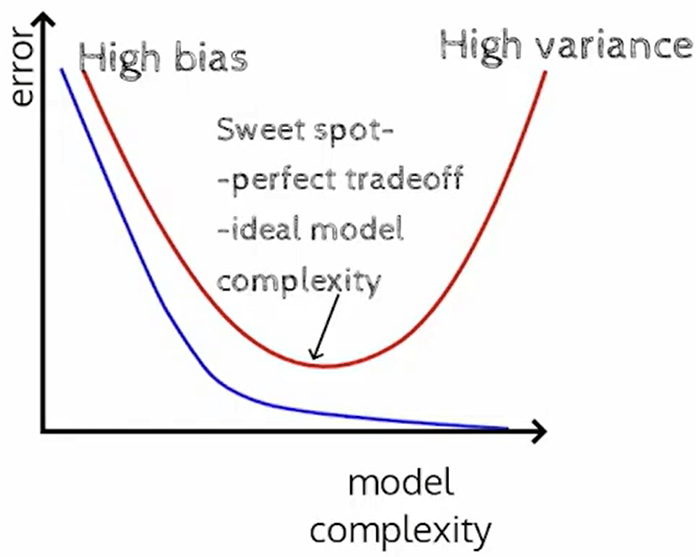
\includegraphics[width=0.5\linewidth]{Degree//static/DL_train_vs_test.png}
        \caption{Train vs Test Error}
        \label{fig:DL-train-vs-test}
    \end{figure}
    \item Complex model is more sensitive to minor changes in the data, as compared to simple models. Hence while training, instead of minimizing the training error we should minimize train error $+\Omega(\theta)$, which is high for complex models and small for simple models.
    \item This is the basis for all the regularization methods.
\end{itemize}

\subsection{Regularization Methods}
\begin{itemize}
    \item For \textbf{L2 Regularization} define the loss as
    \begin{equation*}
        \Bar{L}(w)=L(w)+\frac{\alpha}{2}\lVert w\rVert^2
    \end{equation*}
    and the following gradient would look like
    \begin{equation*}
        \nabla \Bar{L}(w)=\nabla L(w)+\alpha w
    \end{equation*}
    So it is very easy to implement this.
    \item It essentially makes it, so the weights are closer to $0$, non-essential weights will be closer to $0$ as compared to essential weights.
    \item \textbf{Data Augmentation}: Consider images, rotate them, shift them, blur them, change some pixels, etc.
    \item We exploit the fact that certain transformations to the image do not change the label of the image.
    \item Typically, more data = better learning.
    \item Augmentation works well for image classification/object recognition tasks.
    \item It has been shown, that it works well for speech as well.
    \item \textbf{Parameter Sharing} is used in CNNs, essentially same filter is applied at different positions of the image, or same weight matrix acts on different input neurons.
    \item This is typically used in autoencoders, encoder and decoders.
    \item \textbf{Injecting Noise at input}: We can show that for a simple input output neural network, adding Gaussian noise to the input is equivalent to weight decay(L2 regularization).
    \item We essentially shift the input by a slight amount at every epoch, so the model sees a different input at every epoch making it harder to over fit.
    \item This can also be viewed as data augmentation.
    \item We can similarly inject noise at output as well.
    \item \textbf{Early stopping}: Have a patience parameter $p$, after $p$ steps if validation error does not decrease then we stop and return the model $p$ steps before.
    \item This is very effective and widely used, it can be used even with other regularizers.
    \item \textbf{Ensemble Methods}: Combine the output of different models to reduce generalization error. These models can correspond to different classifiers, it could be different instances of the same classifier trained with different hyperparameters, features, samples etc.
    \item \textbf{Bagging}: Form an ensemble using different instances of the same classifier. For a given dataset, construct multiple training sets by sampling with replacement.
    \item Bagging would work well when the errors of the model are independent or uncorrelated, if they are correlated then the mse of the ensemble is as bad as the individual model.
    \item On average, the ensemble will perform at least as well as its individual members.
    \item Training several neural networks for making an ensemble is prohibitively expensive.
    \item \textbf{Dropout}: Refers to dropping out units, temporarily remove a node and all its incoming and outgoing connections resulting in a thinned network.
    \item Each node is retained with a fixed probability, $p=0.5$, for hidden nodes and $p=0.8$ for visible nodes.
    \item We initialize all the parameters of the network and start training. For the first training instance(or mini-batch), we apply dropout resulting in the thinned network. Then update only those parameters that are active.
    \item For the second training instance, we again apply dropout resulting in a different thinned network. We again compute the loss and back propagate.
    \item Each thinned network gets rarely trained but the parameter sharing ensures that no model has untrained or poorly trained parameters.
    \item Dropout essentially applies a masking noise to the hidden units. Prevents hidden units from coadapting.
\end{itemize}

\section{Deep Learning Revival}
\subsection{Unsupervised Pre-Training}
\begin{itemize}
    \item We will first train the weights between the layers using an \textbf{unsupervised objective}, essentially we will try to reconstruct $x$.
    \item If we are able to do this, it would mean that the hidden layers are capturing all the important information of the image. We will be learning one layer at a time.
    \item $h_1$ will try to reconstruct $x$, $h_2$ will try to reconstruct $h_1$, and so on...
    \item After this layerwise pre-training, we add the output layer and train the whole network.
    \item In effect we have initialized the weights of the network using the greedy unsupervised objective and are now fine-tuning these weights using the supervised objective.
    \item This helps in optimization and regularization.
    \item Unsupervised objective ensures that the learning is not greedy w.r.t the supervised objective.
    \item Some other experiments have also shown that pre-training is more robust to random initializations.
    \item This led to people thinking that deep networks are sensitive to initial weights, and maybe if we have better initial weights it would lead to better network.
\end{itemize}

\subsection{Better Activation Functions}
\begin{itemize}
    \item \textbf{Sigmoid}: $\sigma(x)=\frac{1}{1+e^{-x}}$, compresses all its inputs to the range $[0,1]$. $\frac{\partial \sigma(x)}{\partial x}=\sigma(x)(1-\sigma(x))$, once sigmoid neuron is \textbf{saturated}($\sigma(x)=0$ or $1$) then the training will halt as the derivative would become zero.\\
    Another issue is that sigmoid are \textbf{not zero centered}, leading to all positive or all negative gradients, lack of diversity. These are also \textbf{computationally expensive} because of the exponential term.
    \item \textbf{tanh}: $tanh(x)$, compresses all its input to the range $[-1,1]$ so, its \textbf{zero centered}.$\frac{\partial tanh(x)}{\partial x}=(1-tanh^2(x))$, but we still face the issue of \textbf{vanishing gradient}, and it is still \textbf{computationally expensive}.
    \item \textbf{Rectified Linear Unit}: $ReLU(x)=\max{(0,x)}$, does not saturate in the positive region, it is computationally efficient and in practice converges much faster than sigmoid and tanh.\\
    Clearly the derivative is $1$ for $x>0$ and $0$ otherwise, leading to no updates for negative neurons, which makes the neuron dead.\\
    In practice a large fraction of ReLU units can die if the learning rate is set too high.\\
    It is advised to initialize the bias to a positive value.
    \item \textbf{Leaky ReLU}: $f(x)=\max{(0.1x,x)}$, no saturation, computationally efficient, close to zero centered outputs, and will not die.
    \item \textbf{Parametric ReLU}: $f(x)=\max{(\alpha x,x)}$, $\alpha$ can be learned.
    \item \textbf{Exponential Linear Unit}: $ELU=\begin{cases}
        x\text{ if }x>0\\ ae^x-1\text{ if }x\leq 0
    \end{cases}$, close to zero centered outputs, expensive.
    \begin{figure}[H]
        \centering
        \begin{subfigure}[b]{0.3\textwidth}
            \centering
            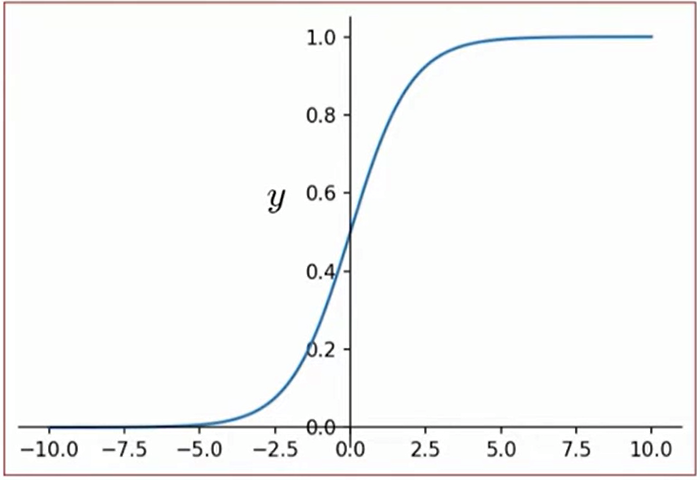
\includegraphics[width=\textwidth]{Degree/static/DL_Sigmoid_function.png}
            \caption{Sigmoid Function}
        \end{subfigure}
        \hfill
        \begin{subfigure}[b]{0.3\textwidth}
            \centering
            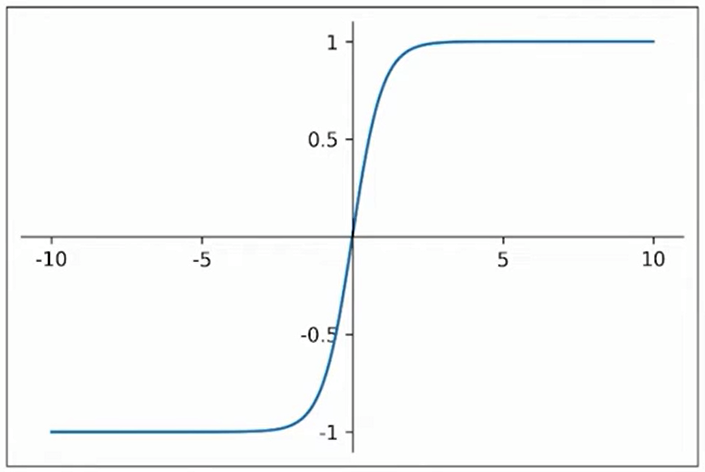
\includegraphics[width=\textwidth]{Degree/static/DL_tanh_function.png}
            \caption{Tanh Function}
        \end{subfigure}
        \hfill
        \begin{subfigure}[b]{0.3\textwidth}
            \centering
            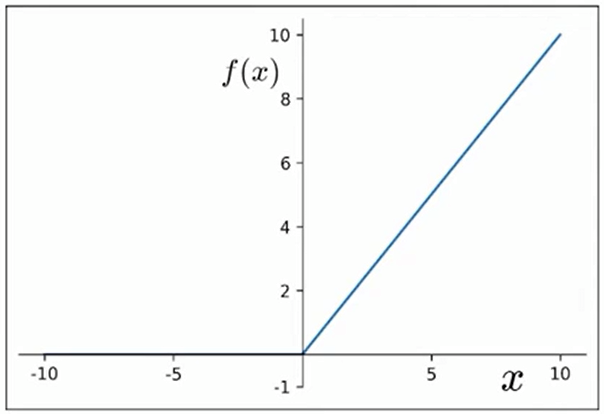
\includegraphics[width=\textwidth]{Degree/static/DL_ReLU_function.png}
            \caption{ReLU Function}
        \end{subfigure}
        \caption{Activation Functions - 1}
    \end{figure}
    \begin{figure}[H]
        \centering
        \begin{subfigure}[b]{0.3\textwidth}
            \centering
            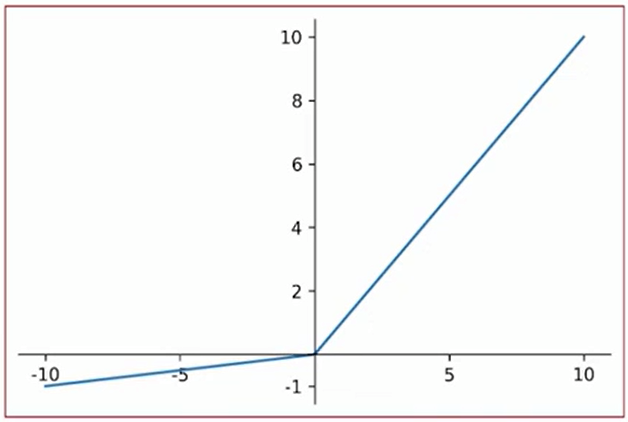
\includegraphics[width=\textwidth]{Degree/static/DL_Leaky_ReLU_function.png}
            \caption{Leaky ReLU Function}
        \end{subfigure}
        \hfill
        \begin{subfigure}[b]{0.3\textwidth}
            \centering
            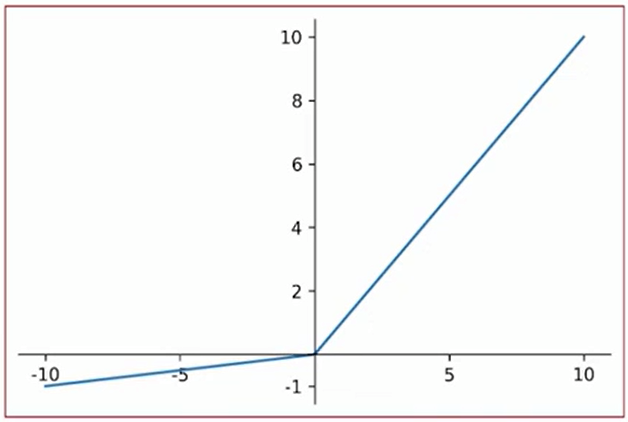
\includegraphics[width=\textwidth]{Degree/static/DL_Leaky_ReLU_function.png}
            \caption{Parametric ReLU Function}
        \end{subfigure}
        \hfill
        \begin{subfigure}[b]{0.3\textwidth}
            \centering
            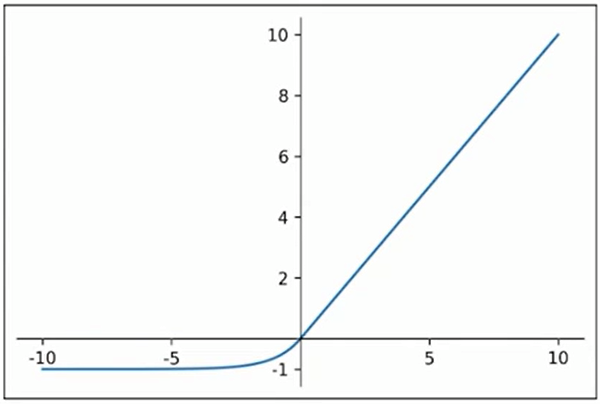
\includegraphics[width=\textwidth]{Degree/static/DL_ELU_function.png}
            \caption{ELU Function}
        \end{subfigure}
        \caption{Activation Functions - 2}
    \end{figure}
    \item \textbf{Model Averaging}: Train $k$ models with independent weights($w_1,w_2,...,w_k$) on independently sampled data points from the original dataset. Each model is expected to be good at predicting a subset of training samples well.\\
    During inference, the prediction is done by averaging the predictions from all the models, it is often \textbf{arithmetic or geometric} mean for regression problems.
    \item In bagging, the subset of training samples seen by each of the models does not change across epochs. Therefore, the model weights get optimized for those samples.
    \item Each sub-model sees only some parts of the training data, therefore we want updates to be larger.
    \item We don't have this luxury in case of dropout.
    \item \textbf{MaxOut}: In a way is a variation of Dropout, but instead of having probability, we take say 3 neurons in a layer and propagate the max of them. Can also be thought of as a generalization of ReLU and Leaky ReLU.\\
    Two MaxOut neurons with sufficient number of affine transformations, act as a universal approximator.
    \item \textbf{Gaussian Error Linear Unit}: $GELU=mx$ where $m\sim Bernoulli(\Phi(x))$
    \item \textbf{Swish}: $x\sigma(\beta x)$, taking $\beta=1.702$ we get GELU, and taking $1$ we get SILU(Sigmoid-weighted Linear Unit).
\end{itemize}

\section{Convolutional Neural Networks}
\begin{itemize}
    \item Convolution operation can be defined as
    \begin{equation*}
        x\ast w=\sum_{a=0}^{\infty}x(t-a)w(a)=\sum_{a=0}^{\infty}x(a)w(t-a)
    \end{equation*}
    where $w$ is called a filter and $x$ is the input.
    \item Similarly 2D convolution operation can be defined as
    \begin{equation*}
        (I\ast K)(i,j)=\sum_{a=0}^{m-1}\sum_{b=0}^{n-1}I(i-a,j-a)K(a,b)
    \end{equation*}
    We can use this for images.
    \item We can define correlation operator as
    \begin{equation*}
        g(i,j)=\sum_{a=0}^{m-1}\sum_{b=0}^{n-1}I(i+a,j+a)K(a,b)
    \end{equation*}
    Correlation and Convolution operator will be same when $K$ is a symmetric matrix.
    \item For practical implementations most libraries implement correlation operator rather than convolution.
    \begin{figure}[H]
        \centering
        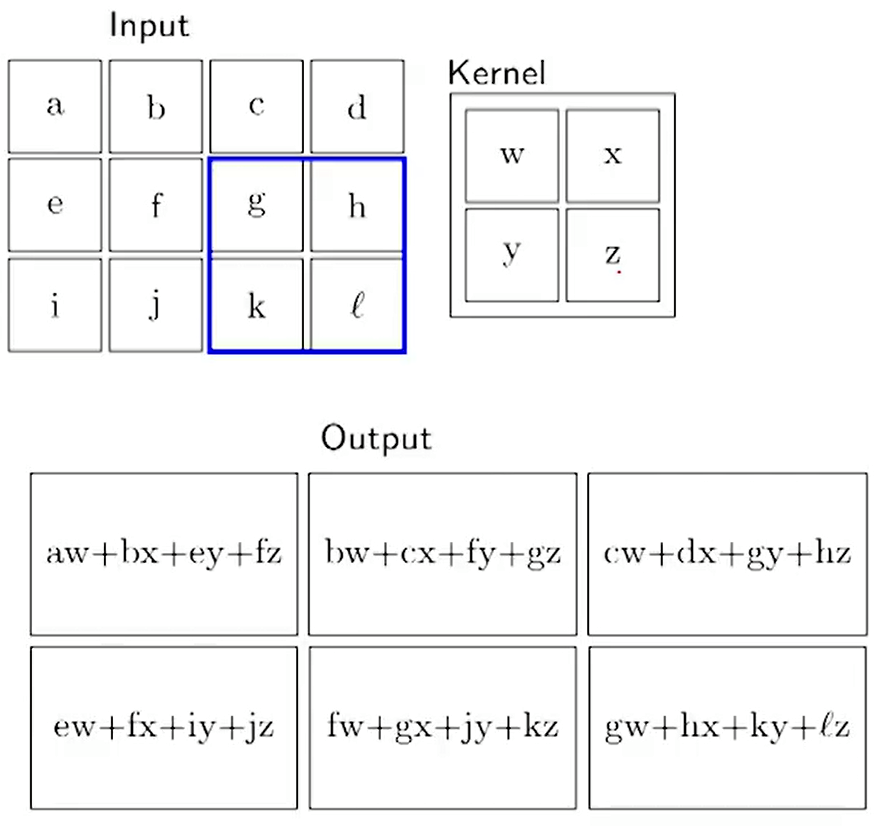
\includegraphics[width=0.5\linewidth]{Degree//static/DL_convolution_example.png}
        \caption{Convolution Example}
    \end{figure}
    \item When we convolve a filter with an image the resulting image is called a feature map.
    \item If we use multiple such filters we will get multiple feature maps, and then we stack them, this number will in a way act as the number of color channels.
    \item Let image be of size $W_1\times H_1\times D_1$, let the number of filters be $K$, let the output be of size $W_2\times H_2\times D_2$, and let stride be $S$ and spatial extent $F$. The filters are of size $F\times F\times D_1$.
    \begin{equation*}
        W_2=1+\frac{W_1-F}{S}\text{     }H_2=1+\frac{H_1-F}{S}\text{     }D_2=K
    \end{equation*}
    \item If we want the output to be of the same size as input, we add padding.
    \begin{equation*}
        W_2=1+\frac{W_1-F+2P}{S}\text{     }H_2=1+\frac{H_1-F+2P}{S}\text{     }D_2=K
    \end{equation*}
    \item One important characteristic of CNNs is \textbf{weight sharing}.
    \item \textbf{Pooling}: Basically the same as a filter, except instead of multiplying with numbers, we take the max/min/average of the pixel intensities within the filter window.
    \item Pooling essentially helps lower the size of the feature maps, and extract only essential or important features.
    \item A simple CNN will have (Convolution$\to$Pooling)$\times 2$ layers, then a normal ANN.
    \item Pooling layers will propagate gradient in backpropagation, as they do not have any weight attached to them.
    \item For Max pooling, the gradient from the next layer is propagated only to the location of the maximum value in the pooling window.
    \item For Average pooling, the gradient from the next layer is distributed equally to all elements in the pooling region because each element contributes equally to the average.
    \item For convolution, the backpropagation update would be convolving the input($X$) to the convolution layer with the loss or gradient values given by the pooling layer.
    \item And when we want to propagate the gradient we will convolve weights($W$) instead of $X$.
\end{itemize}

\subsection{Different Architectures}
\begin{itemize}
    \item \textbf{AlexNet}: Input size is of $227\times 227\times 3$, the architecture can be seen below. Approx $27M$ parameters.
    \begin{figure}[H]
        \centering
        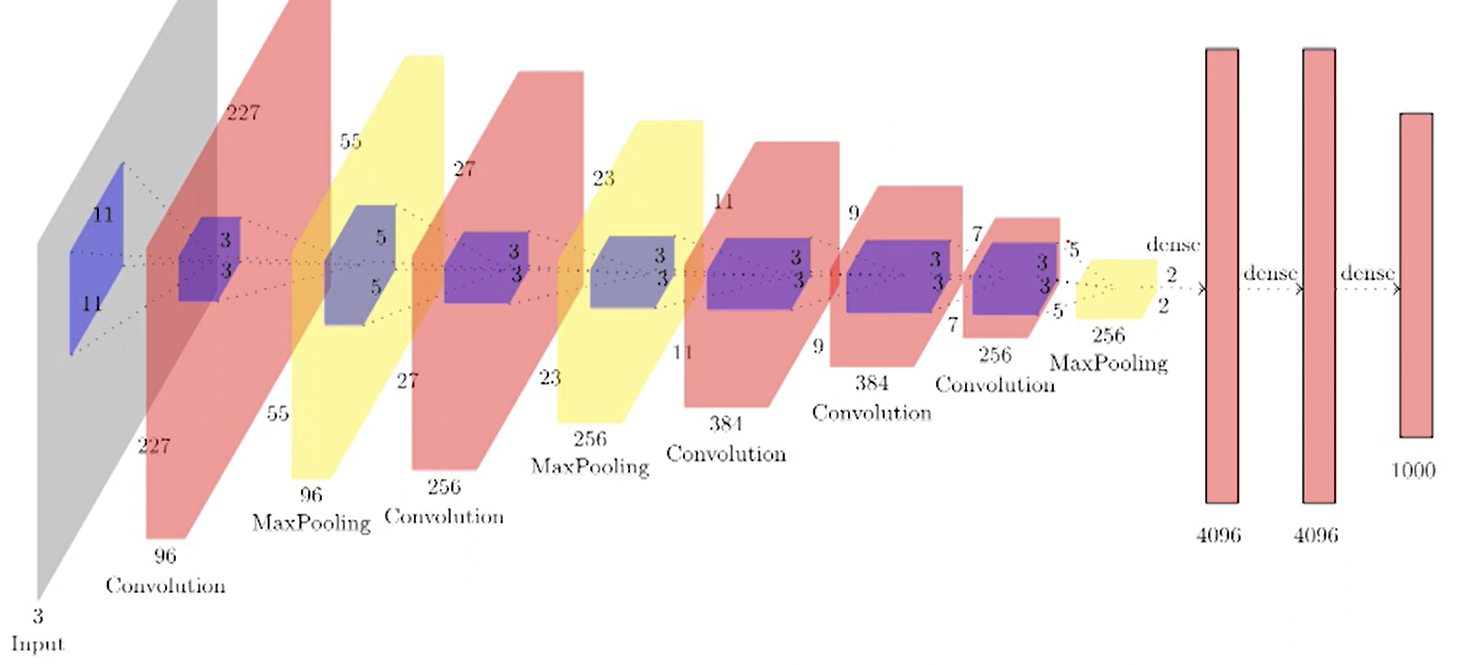
\includegraphics[width=\linewidth]{Degree//static/DL_AlexNet_Architecture.png}
        \caption{AlexNet Architecture}
    \end{figure}
    \item \textbf{ZFNet}: Input size is the same, the architecture is basically the same as AlexNet except the three consecutive convolution layers have filters $512,1024$, $512$ respectively.
    \item \textbf{VGGNet}: Input is again the same, the key idea in this is kernel size is always $3\times 3$.
    \item \textbf{GoogleLeNet}: Key idea is to have multiple sized filters to capture features at varying range.
    \begin{figure}[H]
        \centering
        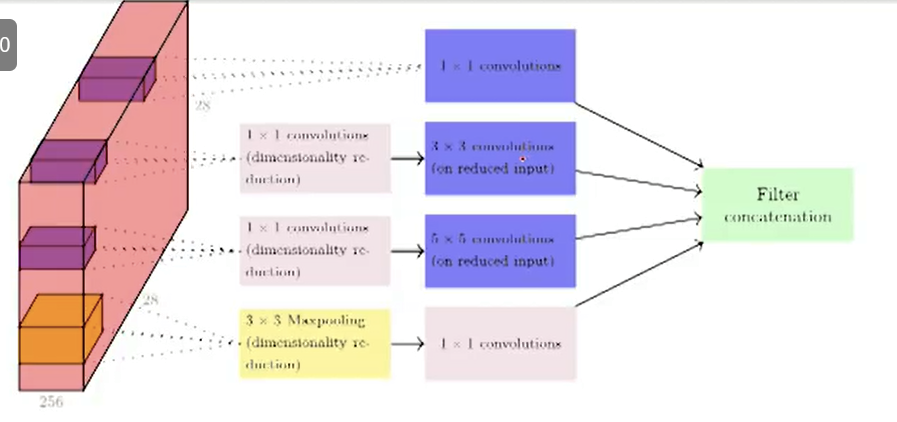
\includegraphics[width=\linewidth]{Degree//static/DL_Inception_Model.png}
        \caption{Inception Model}
    \end{figure}
    \item \textbf{ResNet}: Train a shallow network, then add layers and train deeper network. We can ensure this by adding a skip connection.
\end{itemize}
\pagebreak

\section{Word Representations}
\subsection{Direct Representations}
\begin{itemize}
    \item \textbf{Corpus}: Group of documents.
    \item Consider the set $V$ of all uniques words across all input streams, $V$ is called the \textbf{vocabulary} of the corpus. We need a representation for every word in $V$.
    \item We will be using the following corpus, to understand each representation
    \begin{enumerate}
        \item Human machine interface for computer applications
        \item User opinion of computer system response time
        \item User interface management system
        \item System engineering for improved response time
    \end{enumerate}
    \item Vocabulary for this corpus is $V=[$human, machine, interface, for, computer, applications, user, opinion, of, system, response, time, interface, management, engineering, improved$]$
    \item One very simple way of doing this is to use \textbf{one-hot vectors} of size $|V|$, essentially switch the bit on if the word is present else it is off.
    \item \textbf{machine} would be represented as $\begin{bmatrix}
        0&1&0&...&0&0
    \end{bmatrix}$
    \item $V$ tends to be very large, 50K for PTB, 13M for Google IT corpus.
    \item These representations do not capture any notion of similarity.
    \item With one hot representations, the Euclidean distance between any two words is $\sqrt{2}$ and the cosine similarity between any two words is $0$. 
    \item We want representations of cat and dog to be closer to each other than the representations of cat and truck.
    \item These are also called \textbf{sparse representations}.
    \item A co-ocurrence matrix is a terms $\times$ terms matrix which captures the number of times a term appears in the context of another term
    \item The context is defined as a window of $k$ words around the terms.
    \item With $k=2$, the co-ocurrence matrix for the above corpus would be
    \begin{table}[H]
        \centering
        \begin{tabular}{|c|c|c|c|c|c|c|}
            \hline
             & human & machine & system & for & ... & user \\
             \hline
            human & 0 & 1 & 0 & 1 & ... & 0\\
            \hline
            machine & 1 & 0 & 0 & 1 & ... & 0\\
            \hline
            system & 0 & 0 & 0 & 1 & ... & 2\\
            \hline
            for & 1 & 1 & 1 & 0 & ... & 0\\
            \hline
            .&.&.&.&.&.&.\\
            \hline
            .&.&.&.&.&.&.\\
            \hline
            .&.&.&.&.&.&.\\
            \hline
            user & 0 & 0 & 2 & 0 & ... & 0\\
            \hline
        \end{tabular}
        \caption{Co-Ocurrence Matrix}
    \end{table}
    \item Essentially for the word $w_1$, we check a window of $k$ words around it and count how many times other words appear.
    \item This is also known as a word $\times$ context matrix.
    \item We could choose the set of \textbf{words} and \textbf{contexts} to be same or different.
    \item Each row (column) of the co-ocurrence matrix gives a representation of the corresponding word (context).
    \item Stop words(a, the, for, etc.) are very frequent $\to$ these counts will be very high.
    \item We can solve this by ignoring very frequent words or use a threshold $t$, and if a word, context pair goes above a threshold then we cap it.
    \item Instead of count we can also use PMI
    \begin{equation*}
        PMI(w,c)=\log{\frac{p(c|w)}{p(c)}}=\log{\frac{count(w,c)\cdot N}{count(c)\cdot count(w)}}
    \end{equation*}
    Obviously, when $count(w,c)=0$ then PMI becomes $-\infty$, which is an issue.
    \item We can solve this by taking PMI value as $0$ when $count(w,c)\leq 0$ and using the formula when $count(w,c)> 0$, this is called $PMI_0(w,c)$.
    \item Another solution is instead of $count(w,c)>0$, we replace with $PMI(w,c)>0$. This is called Positive PMI or $PPMI$.
    \begin{table}[H]
        \centering
        \begin{tabular}{|c|c|c|c|c|c|c|}
            \hline
             & human & machine & system & for & ... & user \\
             \hline
            human & 0 & 2.944 & 0 & 2.25 & ... & 0\\
            \hline
            machine & 2.944 & 0 & 0 & 2.25 & ... & 0\\
            \hline
            system & 0 & 0 & 0 & 1.15 & ... & 1.84\\
            \hline
            for & 2.25 & 2.25 & 1.15 & 0 & ... & 0\\
            \hline
            .&.&.&.&.&.&.\\
            \hline
            .&.&.&.&.&.&.\\
            \hline
            .&.&.&.&.&.&.\\
            \hline
            user & 0 & 0 & 1.84 & 0 & ... & 0\\
            \hline
        \end{tabular}
        \caption{PMI Co-Ocurrence Matrix}
    \end{table}
    \item This is however still very large and very sparse, and it grows with vocabulary.
    \item Consider $X=X_{PPMI_{m\times n}}$, we can use singular value decomposition to get a rank $k$ approximation.
    \begin{equation*}
        \hat{X}_{m\times n}=U_{m\times k}\Sigma_{k\times k} V_{k\times n}^T
    \end{equation*}
    \item SVD gives the best rank $k$ approximation of the original data, Discovers latent semantics in the corpus.
    \item SVD will essentially extract the most important features from the matrix.
    \item Conventionally, we take word representation as
    \begin{equation*}
        W_{word}=U\Sigma \in \mathbb{R}^{m\times k}
    \end{equation*}
    This is representation of the $m$ words in the vocabulary and $W_{context}=V$ is taken as the representation of the context words.
    \item This idea comes from the fact that $\hat{X}\hat{X}^T$ and $W_{word}W_{word}^T$ are the same matrices, i.e., they roughly capture the same cosine similarity.
    \item These methods are called count based models because they use the co-ocurrence counts of words. 
\end{itemize}

\subsection{Bag of Words Model}
\begin{itemize}
    \item \textbf{Task}: Predict the $n$th word given previous $n-1$ words.
    \item \textbf{Training data}: All $n$ word windows in the corpus.
    \item Consider doing this for $n=2$, predict the second word given the first.
    \item We can model this problem using a feedforward neural network with one hidden layer. This network will take input a one-hot representation of the context word and output a probability vector of words.
    \item Parameters are $W_{context}\in \mathbb{R}^{k\times |V|}$ and $W_{word}\in \mathbb{R}^{|V|\times k}$, and we use softmax to get probabilities.
    \item The product $W_{context}x$ is simply the $i$th column of $W_{context}$, give $x$ is a one hot vector.
    \item When the $i^{th}$ word is present the $i^{th}$ element in the one hot vector is ON and the $i^{th}$ column of $W_{context}$ gets selected.
    \item There is a one to one correspondence between the words and columns of $W_{context}$.
    \item We can treat the $i^{th}$ column of $W_{context}$ as the representation of the context $i$.
    \item $P(word=i|v)$ depends on the $i^{th}$ column of $W_{word}$.
    \item We thus treat the $i^{th}$ column of $W_{word}$ as the representation of the word $i$.
    \item Consider the context word with index $c$ and the correct output with index $w$
    \begin{equation*}
        \begin{split}
            L(\theta)=-\log \hat{y}_w=-\log P(w|c)\\
            h=W_{context}x_c=u_c\\
            \hat{y}_w=\frac{e^{u_cv_w}}{\sum_{w'\in V}e^{u_cv_{w'}}}
        \end{split}
    \end{equation*}
    $u_c$ is the column of $W_{context}$ corresponding to context word $c$ and $v_w$ is the column of $W_{word}$ corresponding to the word $w$.
    \item Give an context $u_c$ if we are predicting $v_w$ then the update rule for $v_w$ derived from backpropagation is
    \begin{equation*}
        v_w=v_w+\eta u_c(1-\hat{y}_w)
    \end{equation*}
    This increases the cosine similarity between $u_c$ and $v_w$.
    \item The training objective ensures that the cosine similarity between word ($v_w$) and context word ($u_c$) is maximized
    \item In practice, instead of window size of $1$ it is common to use a window size of $d$.
    \item We can simply concatenate all the one-hot representations, and the first layer weights changes to\\
    $[W_{context},W_{context},...d\text{ times}]$, this becomes very complex. Instead, we simply add the column where bit is on.
    \begin{equation*}
        h=\sum_{i=1}^{d-1}u_c,\text{ where }u_c\text{ is the column of }W_{context}\text{ where bit was on}
    \end{equation*}
    \item Computation of softmax is expensive as denominator requires sum of all words in vocabulary.
\end{itemize}

\subsection{Skip Gram Model}
\begin{itemize}
    \item Predicts context words given an input word.
    \item the role of context and word has changed now.
    \item It essentially becomes the same as bag of words, and we run into the same problems.
    \item \textbf{Negative Sampling}
    \item Let $D$ be the set of all correct $(w, c)$ pairs in the corpus
    \item Let $D'$ be the set of all incorrect $(w, r)$ pairs in the corpus
    \item $D'$ can be constructed by randomly sampling a context word $r$ which has never appeared with $w$ and creating a pair $(w, r)$
    \item We are interested in maximizing
    \begin{equation*}
        \prod_{(w,c)\in D}P(z=1|w,c)\prod_{(w,r)\in D'}P(z=0|w,r)=\sum_{(w,c)\in D}\log \sigma(v_c^Tv_w)+\sum_{(w,r)\in D'}\log \sigma(-v_r^Tv_w)
    \end{equation*}
    \item The size of $D'$ is $k$ times the size of $D$.
    \item \textbf{Contrast Estimation}: Consider instead of outputting probability we output a score.
    \item Now, we want the score of correct word $s$ to be higher than wrong word $s_r$, so we try to maximize $s-s_r$.
    \item But we would like the difference to be at least $m$, so we maximize $s-(s_r+m)$
    \item If $s>s_r+m$ then we don't do anything.
    \item \textbf{Hierarchical Softmax}: Construct a binary tree such that there are $|V|$ leaf nodes each corresponding to one word in the vocabulary.
    \item There exists a unique path from the root node to a leaf node.
    \item Let $l(w_1), l(w_2), ..., l(w_p)$ be the nodes on the path from root to $w$
    \item Let $\pi(w)$ be a binary vector such that
    \begin{equation*}
        \pi(w)_k=\begin{cases}
            1,\text{ path branches left at node }l(w_k)\\
            0,\text{ otherwise}
        \end{cases}
    \end{equation*}
    \item Finally each internal node is associated with a vector $u_i$
    \item So the parameters of the module are $W_{context}$ and $u_1, u_2, . . . , u_v$ 
    \item The probability of predicting a word is the same as predicting the correct unique path from the root node to that word.
    \item We model
    \begin{equation*}
        P(\pi(on)_i=1)=\frac{1}{1+e^{-v_c^Tu_i}}\text{ and }P(\pi(on)_i=0)=1-P(\pi(on)_i=1)
    \end{equation*}
    \item Note that $p(w|v_c)$ can now be computed using $|\pi(w)|$ computations instead of $|V|$ required by softmax
    \item Turns out that even a random arrangement of the words on leaf nodes does well in practice.
\end{itemize}

\subsection{GloVe Representations}
\begin{itemize}
    \item Count based methods (SVD) rely on global co-occurrence counts from the corpus for computing word representations
    \item Predict based methods learn word representations using co-occurrence information
    \item We will now combine the two.
    \item Consider $X$ as the SVD decomposed matrix of the previous corpus.
    \item $X_{ij}$ encodes important global information about the co-occurrence between $i$ and $j$.
    \item Now we enforce
    \begin{equation*}
        \begin{split}
            &v_i^Tv_j=\log P(j|i)=\log X_{ij}-\log X_i\\
            &v_j^Tv_i=\log X_{ji}-\log X_j=\log X_{ij}-\log X_j(X_{ij}=X_{ji})
        \end{split}
    \end{equation*}
    \item Adding the two equations we get
    \begin{equation*}
        \begin{split}
            &2v_i^Tv_j=2\log X_{ij}-\log X_i-\log X_j\\
            &v_i^Tv_j=\log X_{ij}-\frac{1}{2}\log X_i-\frac{1}{2}\log X_j=\log X_{ij}-b_i-b_j\\
            &v_i^Tv_j+b_i+b_j=\log X_{ij}\\
            &\min_{v_i,v_j,b_i,b_j}\sum_{i,j}(v_i^Tv_j+b_i+b_j-\log X_{ij})^2 
        \end{split}
    \end{equation*}
    where $v_i^Tv_j+b_i+b_j$ is the predicted value using model parameters and $\log X_{ij}$ is the actual value calculated from the given corpus.
    \item One drawback is that, this weighs all co-occurrences equally.
    \item A simple fix is to multiply a weighing function $f(X_{ij})$
    \begin{equation*}
        f(x)=\begin{cases}
            (\frac{x}{x_{max}})^\alpha,\text{ if }x<x_{max}\\
            1,\text{ otherwise}
        \end{cases}
    \end{equation*}
    where $\alpha$ can be tuned for a given dataset.
\end{itemize}

\subsection{Evaluating Word Representations}
\begin{itemize}
    \item \textbf{Semantic Relatedness}
    \begin{enumerate}
        \item Ask humans to judge the relatedness between a pair of words
        \item Compute the cosine similarity between the corresponding word vectors learned by the model
        \item Given many such word pairs, compute the correlation between $S_{model}$ \& $S_{human}$, and compare different models
        \item Model 1 is better than Model 2 if $correlation(S_{model1}, S_{human}) > correlation(S_{model2}, S_{human})$
    \end{enumerate}
    \item \textbf{Synonym Detection}
    \begin{enumerate}
        \item Given: a term and four candidate synonyms
        \item Pick the candidate which has the largest cosine similarity with the term
        \item Compute the accuracy of different models and compare
    \end{enumerate}
\end{itemize}

\section{Sequential Learning}
\subsection{Introduction}
\begin{itemize}
    \item In many applications the input is not of a fixed size
    \item Further successive inputs may not be independent of each other
    \item We need to look at a sequence of (dependent) inputs and produce an output (or outputs)
    \item Each input corresponds to one time step
    \item Consider the task of predicting the part of speech tag (noun, adverb, adjective verb) of each word in a sentence
    \item Once we see an adjective (social) we are almost sure that the next word should be a noun (man)
    \item Thus the current output (noun) depends on the current input as well as the previous input
    \item Further the size of the input is not fixed (sentences could have a arbitrary number of words)
    \item Notice that here we are interested in producing an output at each time step
    \item Each network is performing the same task (input : word, output : tag)
    \item Sometimes we may not be interested in producing an output at every stage
    \item Instead we would look at the full sequence and then produce an output
    \item consider the task of predicting the polarity of a movie review
    \item The prediction clearly does not depend only on the last word but also on some words which appear before
    \item Here again we could think that the network is performing the same task at each step (input : word, output : $+/-$) but it’s just that we don’t care about intermediate outputs
    \item Sequences could be composed of anything (not just words)
\end{itemize}

\subsection{Recurrent Neural Networks}
\begin{itemize}
    \item The function being executed at each time step is
    \begin{equation*}
        \begin{split}
            &s_i=\sigma(Ux_i+b)\\
            &y_i=O(Vs_i+c)
        \end{split}
    \end{equation*}
    where $i$ is the timestep
    \item Since we want the same function to be executed at each timestep we should share the same network
    \item This parameter sharing also ensures that the network becomes agnostic to the size of the input
    \item Since we are simply going to compute the same function at each timestep, the number of timesteps doesn’t matter
    \item We just create multiple copies of the network and execute them at each timestep
    \item Consider that we feed all previous inputs to the current network, this will be infeasible as now the network does not compute the same function at each time step and hence parameter sharing cannot take place.
    \item The solution is to add a recurrent connection in the network
    \begin{equation*}
        \begin{split}
            &s_i=\sigma(Ux_i+Ws_{i-1}+b)\\
            &y_i=O(Vs_i+c)
        \end{split}
    \end{equation*}
    \item This can be represented as follows
    \begin{figure}[H]
        \centering
        \begin{subfigure}[b]{0.45\textwidth}
            \centering
            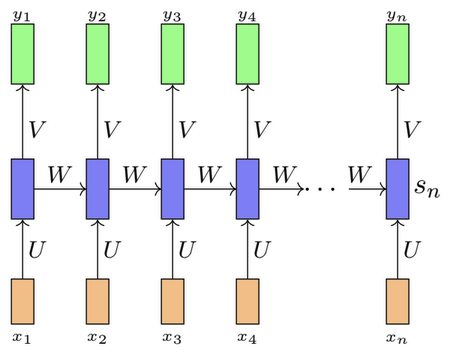
\includegraphics[width=\textwidth]{Degree/static/DL_RNN.png}
        \end{subfigure}
        \begin{subfigure}[b]{0.45\textwidth}
            \centering
            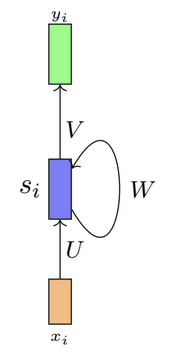
\includegraphics[width=0.37\textwidth]{Degree/static/DL_compact_RNN.png}
        \end{subfigure}
        \caption{Recurrent Neural Network}
    \end{figure}
    \item Consider $x_i\in \mathbb{R}^n$, $s_i\in \mathbb{R}^d$ and $y_i\in \mathbb{R}^k$, then the dimensions of the parameters are
    \begin{equation*}
        U\in \mathbb{R}^{n\times d}\text{  }V\in \mathbb{R}^{d\times k}\text{ and }W\in \mathbb{R}^{d\times d}
    \end{equation*}
    \item The total loss is simply the sum of loss over all time steps.
    \item The gradient of $V$ and $U$ is straightforward backpropagation.
    \item However, gradient of $W$ will be a chain of gradients going through time, aka backpropagation through time.
    \item For $W$ there is a high chance of vanishing/exploding gradients, as such we restrict backprop time steps to $\tau$.
    \item The state ($s_i$) of an RNN records information from all previous time steps
    \item At each new timestep the old information gets morphed by the current input
    \item One could imagine that after $t$ steps the information stored at time step $t-k$ gets completely morphed so much that it would be impossible to extract the original information stored at time step $t - k$.
    \item A similar problem occurs when the information flows backwards
    \item It is very hard to assign the responsibility of the error caused at time step $t$ to the events that occurred at time step $t - k$
\end{itemize}

\subsection{Long Short Term Memory}
\begin{itemize}
    \item Consider the task of predicting the sentiment of a review
    \item RNN reads the document from left to right and after every word updates the state
    \item By the time we reach the end of the document the information obtained from the first few words is completely lost
    \item Ideally we want to
    \begin{enumerate}
        \item forget the information added by stop words
        \item selectively read the information added by
        previous sentiment bearing words
        \item selectively write new information from the current word to the state
    \end{enumerate}
    \item we have computed a state $s_{t-1}$ at timestep $t - 1$, and now we want to overload it with new information ($x_t$) and compute a new state ($s_t$).
    \item We introduce a vector $o_{t-1}$ which decides what fraction of each element of $s_{t-1}$ should be passed to the next state
    \item Each element of $o_{t-1}$ gets multiplied with the corresponding element of $s_{t-1}$
    \item Each element of $o_{t-1}$ is restricted to be between $0$ and $1$
    \begin{equation*}
        \begin{split}
            &o_{t-1}=\sigma(W_oh_{t-2}+U_ox_{t-1}+b_o)\\
            &h_{t-1}=o_{t-1}\odot \sigma(s_{t-1})
        \end{split}
    \end{equation*}
    $W_o,U_o,b_o$ need to be learned.
    \item $o_t$ is called the output gate as it decides how much to pass (write) to the next time step
    \item Now we calculate state information as
    \begin{equation*}
        \Tilde{s}_t=\sigma(Wh_{t-1}+Ux_t+b)
    \end{equation*}
    \item However, we may not want to use all this new information and only selectively read from it before constructing the new cell state $s_t$
    \item To do this we introduce another gate called the input gate
    \begin{equation*}
        i_t=\sigma(W_ih_{t-1}+U_ix_t+b_i)
    \end{equation*}
    and then take dot product to get new temporary state $\Tilde{s}_t$
    \item To selectively forget, we introduce another forget gate
    \begin{equation*}
        f_t=\sigma(W_fh_{t-1}+U_fx_t+b_f)
    \end{equation*}
    \item Now we have the full set of equations for LSTM, the gates are
    \begin{equation*}
        \begin{split}
            &o_t=\sigma(W_oh_{t-1}+U_ox_t+b_o)\\
            &i_t=\sigma(W_ih_{t-1}+U_ix_t+b_i)\\
            &f_t=\sigma(W_fh_{t-1}+U_fx_t+b_f)
        \end{split}
    \end{equation*}
    and the state equations are
    \begin{equation*}
        \begin{split}
            &\Tilde{s}_t=\sigma(Wh_{t-1}+Ux_t+b)\\
            &s_t=f_t\odot s_{t-1}+i_t\odot \Tilde{s}_t\\
            &h_t=o_t\odot \sigma(s_t)\text{ and }rnn_{output}=h_t
        \end{split}
    \end{equation*}
    \begin{figure}[H]
        \centering
        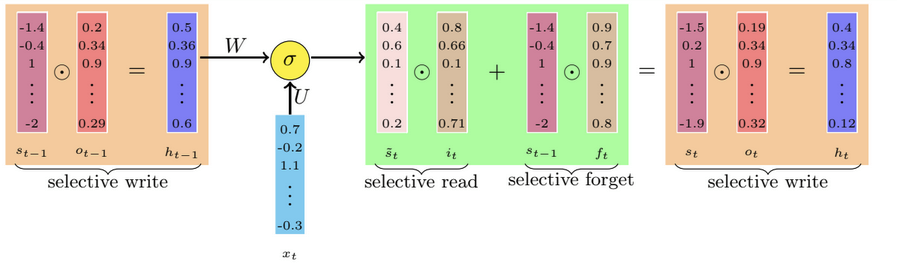
\includegraphics[width=0.8\linewidth]{Degree//static/DL_LSTM.png}
        \caption{Long Short Term Memory}
    \end{figure}
    \item Another variant of LSTM is Gated Recurrent Unit, which has the following set of equations
    \begin{equation*}
        \begin{split}
            &o_t=\sigma(W_os_{t-1}+U_ox_t+b_o)\\
            &i_t=\sigma(W_is_{t-1}+U_ix_t+b_i)\\
            &\Tilde{s}_t=\sigma(W(o_t\odot s_{t-1})+Ux_t+b)\\
            &s_t=(1-i_t)\odot s_{t-1}+i_t\odot \Tilde{s}_t
        \end{split}
    \end{equation*}
    \item No explicit forget gate, the forget gate and input gates are tied.
    \item During forward propagation, the gates control the flow of information
    \item They prevent any irrelevant information from being written to the state
    \item Similarly, during backward propagation they control the flow of gradients
    \item It is easy to see that during backward pass the gradients will get multiplied by the gate
    \item If the state at time $t-1$ did not contribute much to the state at time $t$ then during backpropagation the gradients flowing into $s_{t-1}$ will vanish
    \item But this kind of vanishing gradient is fine, since $s_{t-1}$ did not contribute to $s_t$ we don’t want to hold it responsible for the crimes of $s_t$
\end{itemize}

\section{Encoder-Decoder Models}
\subsection{Introduction}
\begin{itemize}
    \item What if we want to generate a sentence given an image?
    \item We are now interested in $P(y_t|y_{t-1},I)$ instead of $P(y_t|y_{t-1})$, where $I$ is an image.
    \item We could now model $P(y_t = j|y_{t-1},I)$ as $P(y_t=j|s_t,f_{c_7}(I))$ where $f_{c_7}(I)$ is the representation obtained from the convolution layer of an image
    \item There are many ways of making $P(y_t = j)$ conditional on $f_{c_7}(I)$
    \item \textbf{Option 1}: Set $s_0 = f_{c_7}(I)$
    \item Now $s_0$ and hence all subsequent $s_t$’s depend on $f_{c_7}(I)$
    \item We can thus say that $P(y_t = j)$ depends on $f_{c_7}(I)$
    \item \textbf{Option 2}: Another more explicit way of doing this is to compute
    \begin{equation*}
        s_t=RNN(s_{t-1},[x_t,f_{c_7}(I)])
    \end{equation*}
    \item We are explicitly using $f_{c_7}(I)$ to compute $s_t$ and hence $P(y_t = j)$
    \item A CNN is first used to encode the image
    \item A RNN is then used to decode (generate) a sentence from the encoding
    \item This is a typical encoder decoder architecture
    \item Both the encoder and decoder use a neural network
    \item Alternatively, the encoder’s output can be fed to every step of the decoder
    \begin{figure}[H]
        \centering
        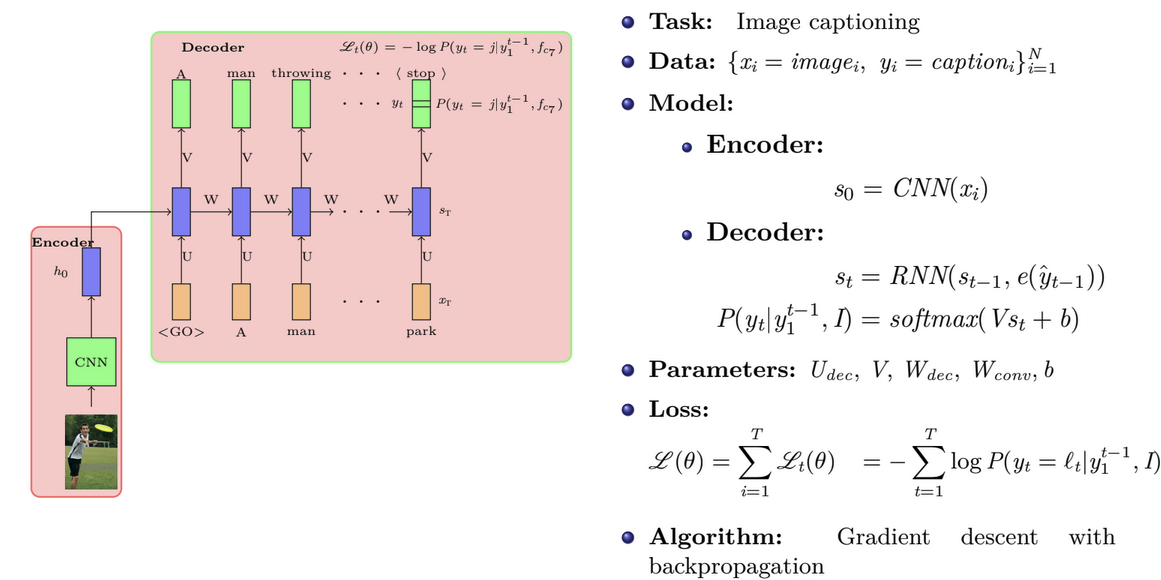
\includegraphics[width=0.8\textwidth]{Degree//static/DL_encoder_decoder.png}
        \caption{Image Captioning}
    \end{figure}
    \begin{figure}[H]
        \centering
        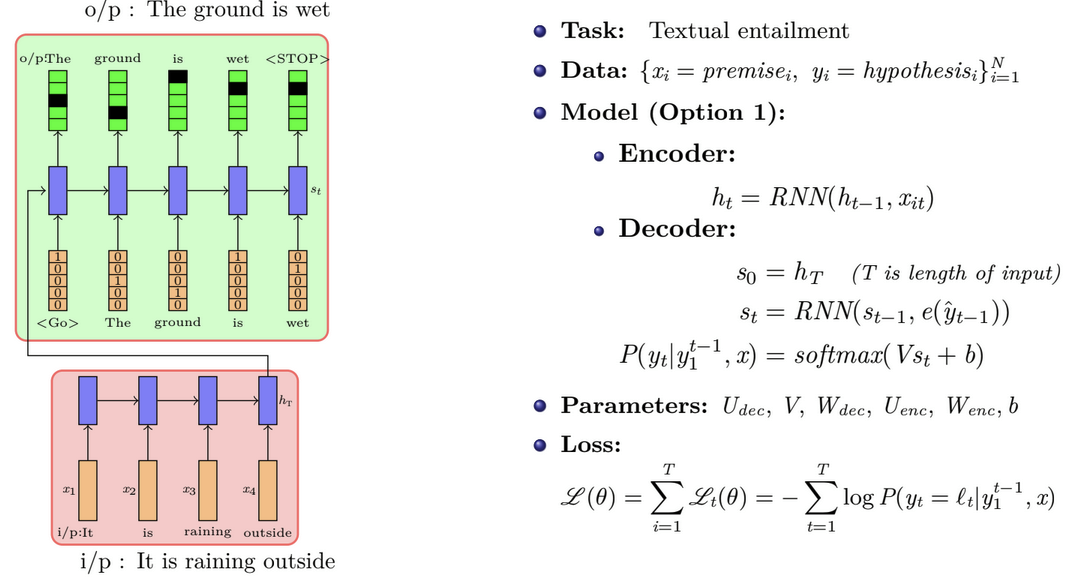
\includegraphics[width=0.8\textwidth]{Degree/static/DL_Encoder_decoder_1.png}
        \caption{Textual Entailment}
    \end{figure}
    \begin{figure}[H]
        \centering
        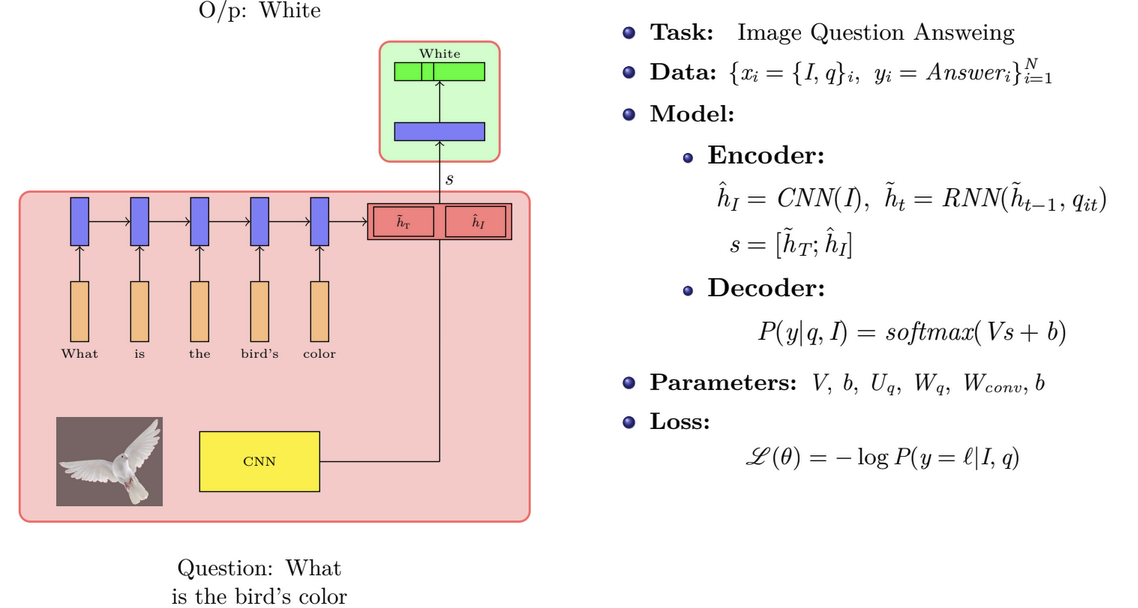
\includegraphics[width=0.8\textwidth]{Degree/static/DL_Encoder_decoder_2.png}
        \caption{Image Question Answering}
    \end{figure}
    \begin{figure}[H]
        \centering
        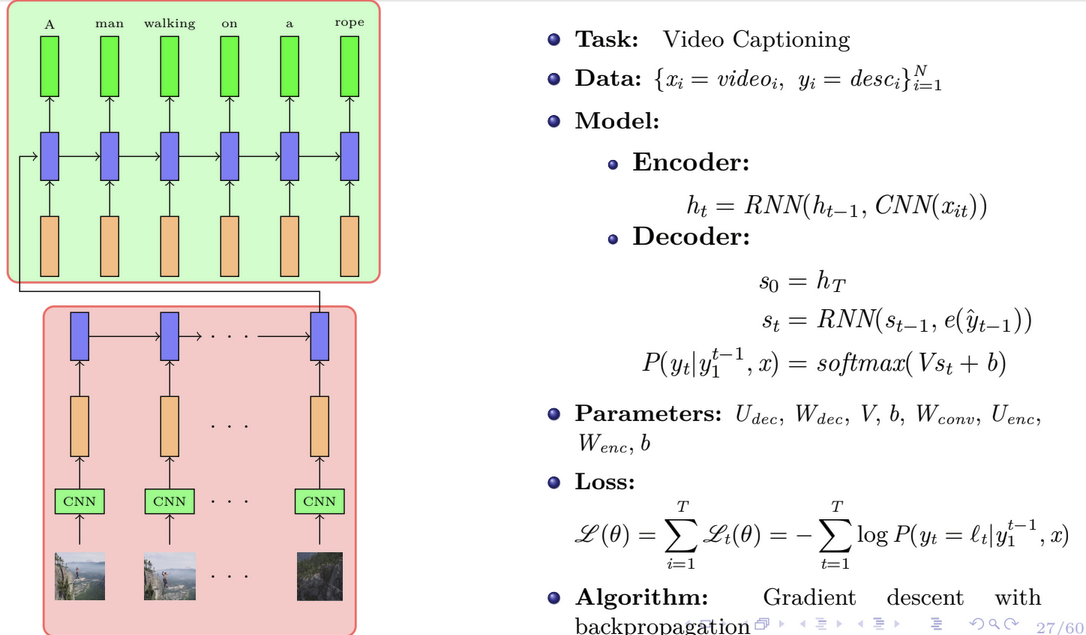
\includegraphics[width=0.7\textwidth]{Degree/static/DL_encoder_decoder_3.png}
        \caption{Video Captioning}
    \end{figure}
\end{itemize}

\subsection{Attention Mechanism}
\begin{itemize}
    \item Encoder decoder models can be made even more expressive by adding an “attention” mechanism
    \item At each time-step we should feed only this relevant information (i.e. encodings of relevant words) to the decoder
    \item We could just take a weighted average of the corresponding word representations and feed it to the decoder.
    \item The machine will have to learn this from the data
    \item To enable this, we define a function $e_{jt} = f_{ATT}(s_{t-1}, h_j)$
    \item This quantity captures the importance of the $j^{th}$ input word for decoding the $t^{th}$ output word.
    \item We can normalize these weights by using the softmax function
    \begin{equation*}
        \alpha_{jt}=\frac{\exp{e^{jt}}}{\sum_{j=1}^M\exp{e^{jt}}}
    \end{equation*}
    \item $\alpha_{jt}$ denotes the probability of focusing on the $j^{th}$ word to produce the $t^{th}$ output word.
    \item One possible choice for $f_{ATT}$ is
    \begin{equation*}
        e_{jt}=V_{att}^T\tanh{U_{att}s_{t-1}+W_{att}h_j}
    \end{equation*}
    \item We are essentially asking the model to approach the problem in a better, more natural way
    \begin{figure}[H]
        \centering
        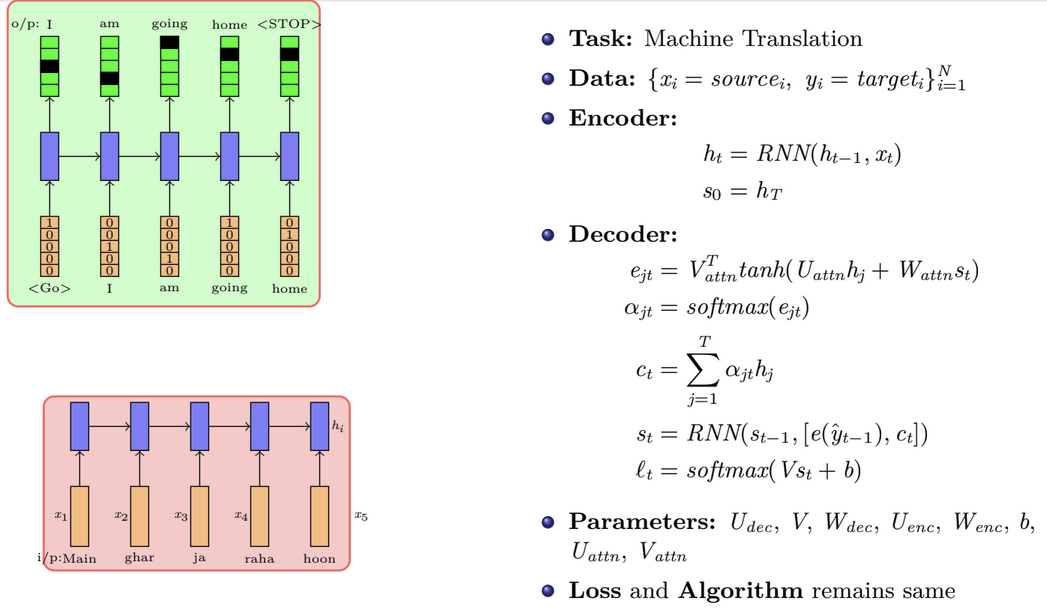
\includegraphics[width=0.8\linewidth]{Degree//static/DL_machine_translation_attention.png}
        \caption{Architecture with Attention}
    \end{figure}
    \item We can check whether the attention model learns something meaningful by plotting the attention weights as a heatmap.
    \item In the case of text, we have a representation for every location of the input sequence.
    \item But for images, we typically use representation from one of the fully connected layers. This representation does not contain any location information.
    \item Instead of the $f_{c_7}$ representation, we use the output of one of the convolution layers, which has spatial information.
    \item For example, the output of the $5^{th}$ convolutional layer of VGGNet is a $14 \times 14 \times 512$ size feature map. We could think of this as $196$ locations, each having a $512$ dimensional representation. The model will then learn an attention over these locations.
\end{itemize}

\subsection{Hierarchical Attention}
\begin{itemize}
    \item Consider a dialog between a user (u) and a bot (B)
    \item The dialog contains a sequence of utterances between the user and the bot
    \item Each utterance in turn is a sequence of words
    \item Thus what we have here is a “sequence of sequences” as input.
    \item We could think of a two level hierarchical RNN encoder
    \item The first level RNN operates on the sequence of words in each utterance and gives us a representation
    \item We now have a sequence of utterance representations (red vectors in the image)
    \item We can now have another RNN which encodes this sequence and gives a single representations for the sequences of utterances
    \item The decoder can then produce an output sequence conditioned on this utterance
    \begin{figure}[H]
        \centering
        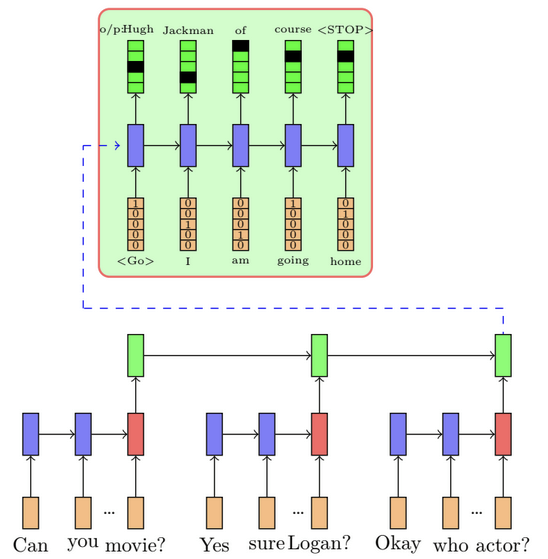
\includegraphics[width=0.5\linewidth]{Degree//static/DL_2_layer_RNN.png}
        \caption{Two layer RNN}
    \end{figure}
    \item Consider another example of classification of documents, each document is a sequence of sentences and each sentence is in turn a sequence of words.
    \begin{figure}[H]
        \centering
        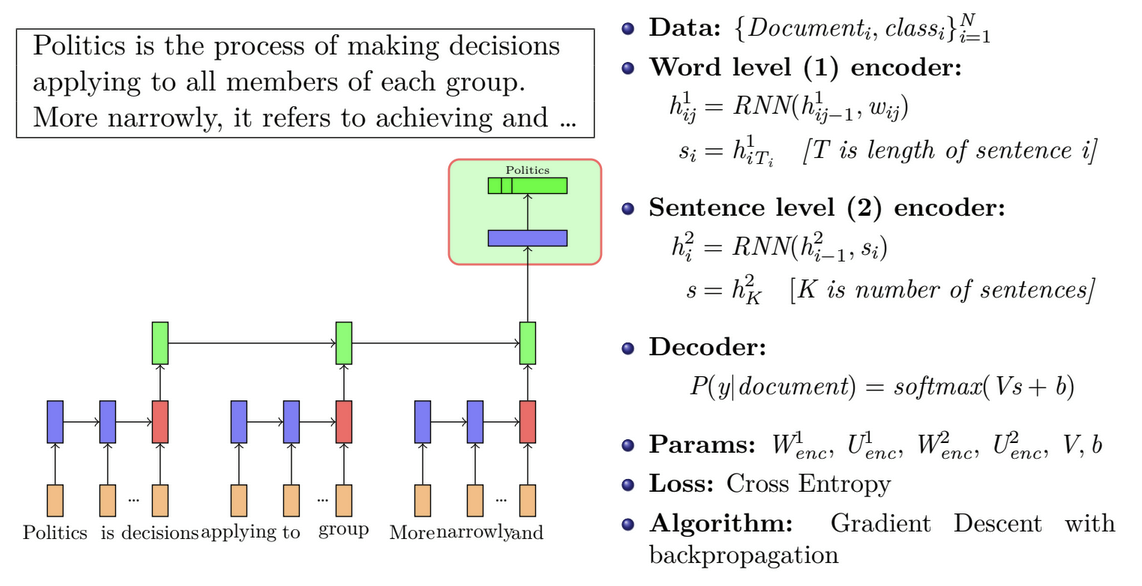
\includegraphics[width=0.8\linewidth]{Degree//static/DL_document_classification.png}
        \caption{Document Classification}
    \end{figure}
    \item We need attention at two levels\\
    First, we need to attend to important (most informative) words in a sentence.\\
    Then we need to attend to important (most informative) sentences in a document.
    \begin{figure}[H]
        \centering
        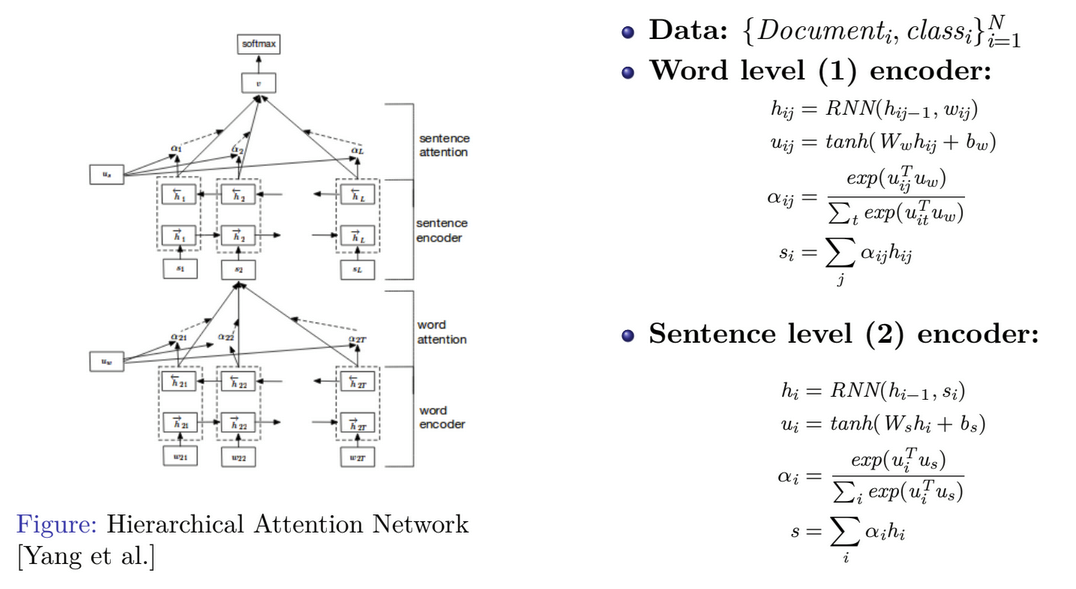
\includegraphics[width=\linewidth]{Degree//static/DL_transformer_encoder.png}
        \caption{Encoder Architecture}
    \end{figure}
    \begin{figure}[H]
        \centering
        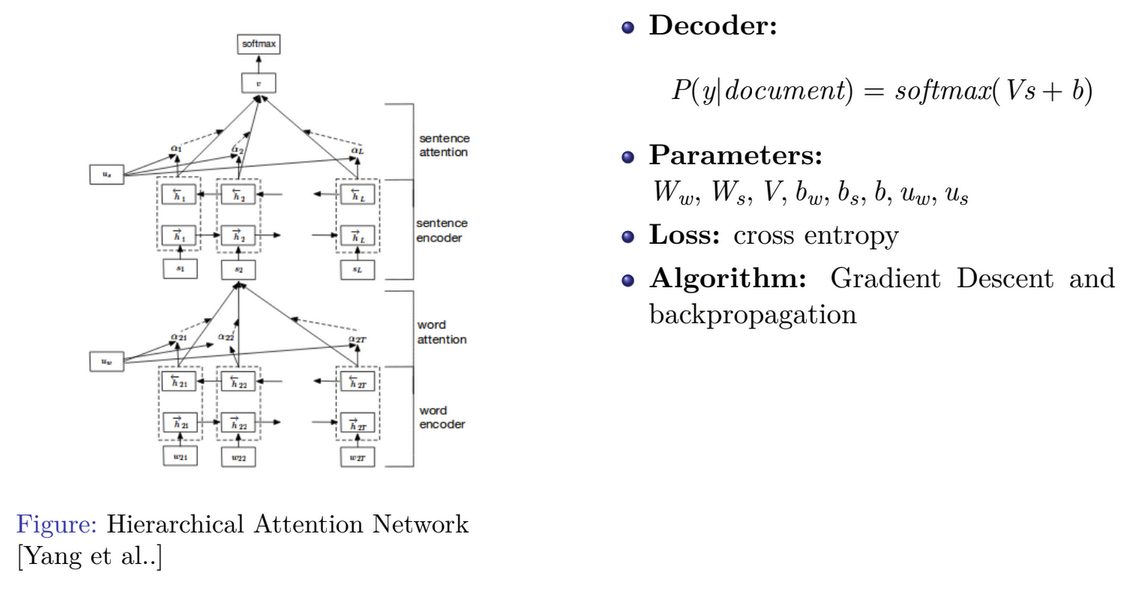
\includegraphics[width=\linewidth]{Degree//static/DL_transformer_decoder.png}
        \caption{Decoder Architecture}
    \end{figure}
\end{itemize}
\pagebreak

\section{Transformer Models}
\begin{itemize}
    \item In encoder-decoder architecture, we have to wait for until $s_{t-1}$ is calculated to calculate $s_t$.
    \item The idea is to calculate all these in parallel, instead of waiting.
    \begin{figure}[H]
        \centering
        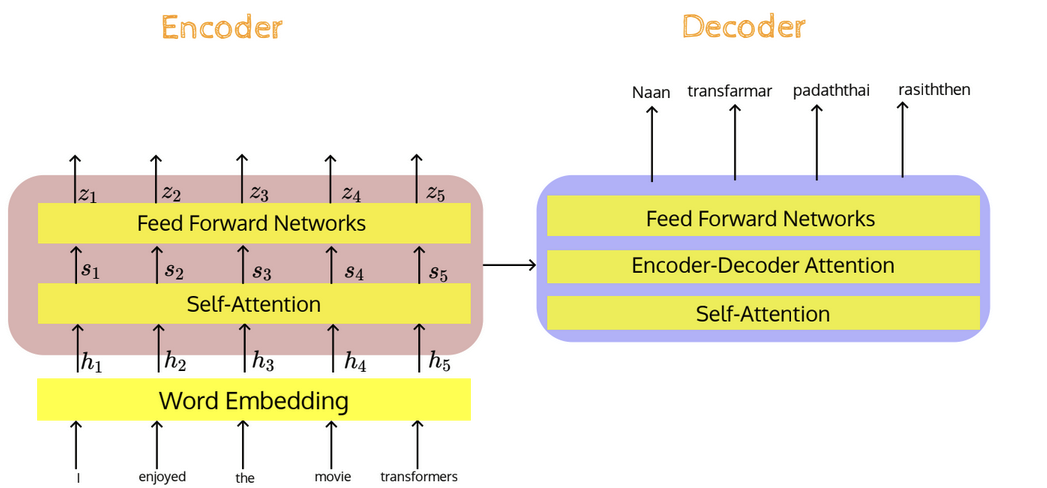
\includegraphics[width=0.8\linewidth]{Degree//static/DL_transformer_architecture.png}
        \caption{Transformer Architecture}
    \end{figure}
\end{itemize}
\subsection{Self-Attention}
\begin{itemize}
    \item Inputs are vectors, word embeddings, and the outputs are also vectors.
    \item Given a word in a sentence, we want to compute the relational score between the word and the rest of the words in the sentence, such that the score is higher if they are related contextually.
    \item now both the vectors $s_i$ and $h_j$, for all $i,j$ are available for all the time.
    \item The score function we used was
    \begin{equation*}
        score(s_{t-1},h_j)=V_{att}^T\tanh{U_{att}s_{t-1}W_{att}h_j}
    \end{equation*}
    \item There are three vectors involved in computing the score at each time step.
    \item We get them by transforming $h_j$
    \item $q_j=W_Qh_j$, called the query vector
    \item $k_j=W_Kh_j$ called the key vector
    \item $v_j=W_Vh_j$ called the value vector
    \begin{figure}[H]
        \centering
        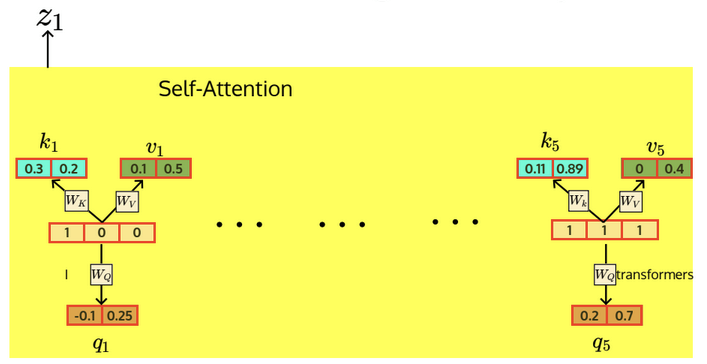
\includegraphics[width=0.8\linewidth]{Degree//static/DL_self_attention.png}
        \caption{Self Attention}
    \end{figure}
    \item We will first calculate $score(q_1,k_j)$, $e_{1j}=[q_1\cdot k_1,q_1\cdot k_2,...,q_1\cdot k_5]$
    \item Then we get $\alpha_{1j}=softmax(e_{1j})$, finally we get $z_1=\sum_{j=1}^5\alpha_{1j}v_j$
    \item Query and key vector participate in calculating $\alpha$, and value vector will participate in getting final output.
    \item All query, key and value vectors can be computed in one go, as follows
    \begin{equation*}
        Q=[q_1,q_2,...,q_T]=W_Q[h_1,h_2,...,h_T]
    \end{equation*}
    \item The entire output can also be computed in parallel as follows
    \begin{equation*}
        Z=[z_1,z_2,...,z_T]=softmax(\frac{Q^TK}{\sqrt{d_k}})V^T
    \end{equation*}
    where $d_k$ is the dimension of key vector.
    \begin{figure}[H]
        \centering
        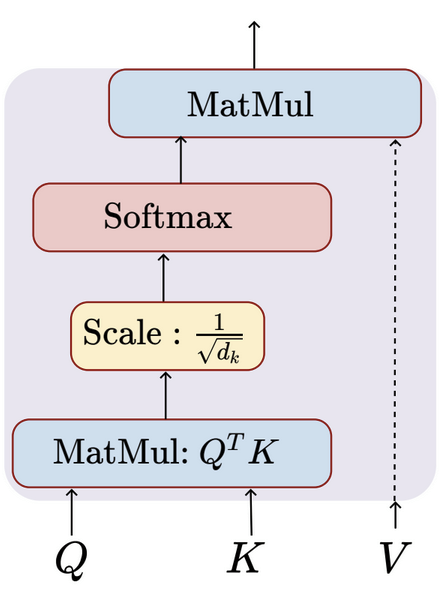
\includegraphics[width=0.3\linewidth]{Degree//static/DL_self_attention_block.png}
        \caption{Self Attention Block}
    \end{figure}
\end{itemize}

\subsection{Multi-Headed Attention}
\begin{itemize}
    \item The idea of having multi-headed attention is pretty much the same idea for having multiple filters in CNN.
    \item \textbf{Two-headed attention}: Have two self attention block side-by-side.
    \item We simply concatenate the output from each block.
    \begin{figure}[H]
        \centering
        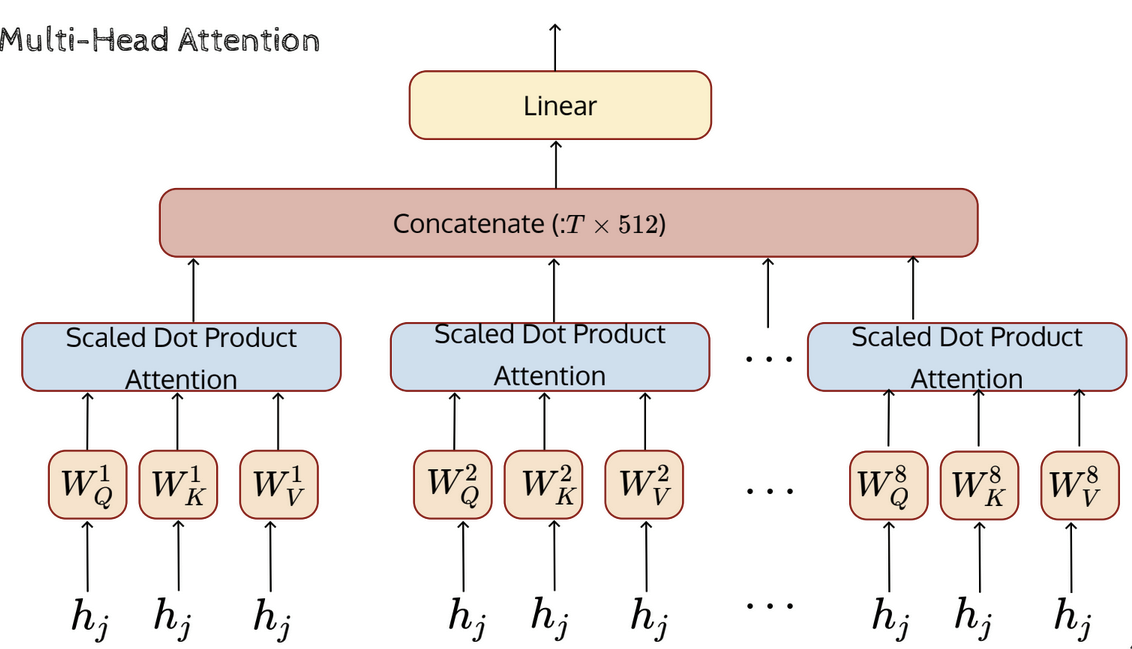
\includegraphics[width=0.8\linewidth]{Degree//static/DL_multi_head_attention.png}
        \caption{Multi-Headed Attention Block}
    \end{figure}
    \item The outputs are then passed to a feed forward network, this is our usual ANN.
    \begin{figure}[H]
        \centering
        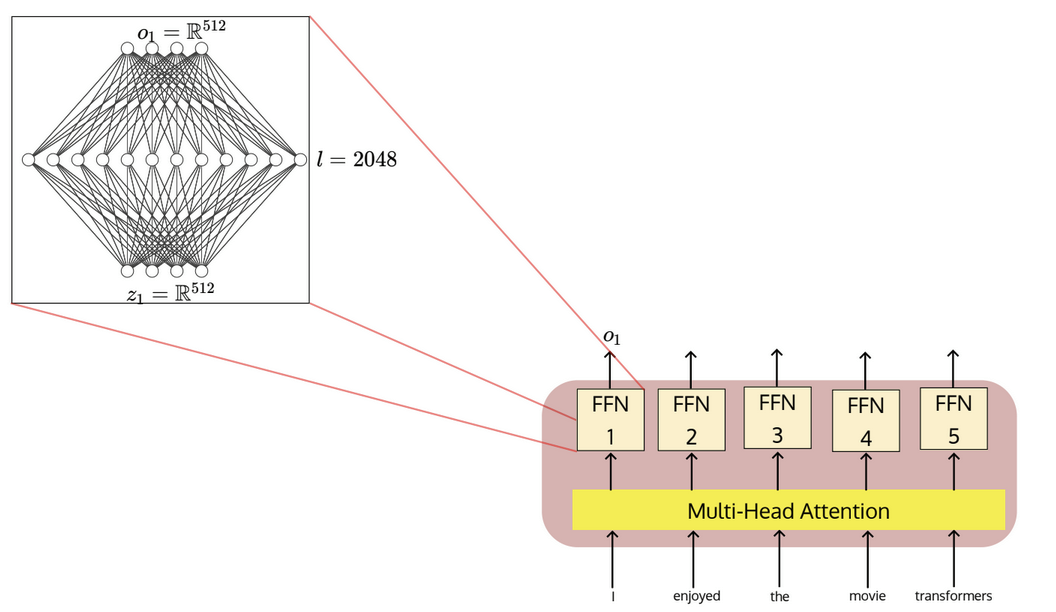
\includegraphics[width=0.8\linewidth]{Degree//static/DL_feed_forward_network.png}
        \caption{Feed Forward Network}
    \end{figure}
    \item Identical network for each position, $FFN(z) = \max(0, W_1z + b_1)W_2 + b_2$
    \item The encoder is composed of identical layers, and each layer is composed of 2 sub-layers.
    \item The computation is parallelized in the horizontal direction, i.e. within a training sample, of the encoder stack, not along the vertical direction.
    \begin{figure}[H]
        \centering
        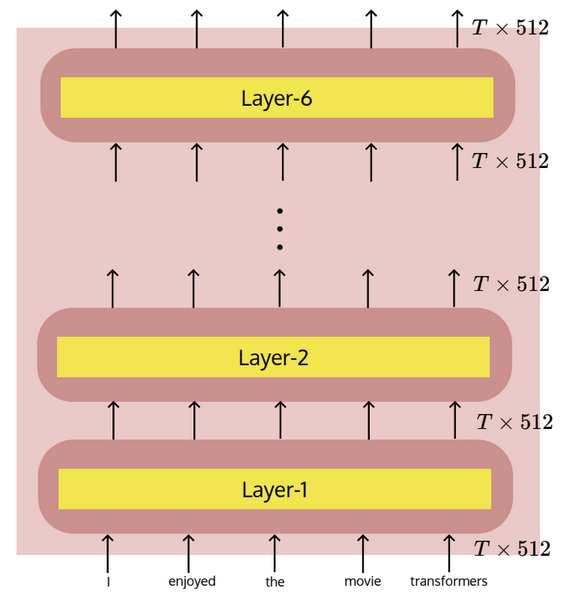
\includegraphics[width=0.5\linewidth]{Degree//static/DL_encoder_stack.png}
        \caption{Encoder Stack}
    \end{figure}
\end{itemize}

\subsection{Decoder Architecture}
\begin{itemize}
    \item Takes input from the encoder, and also has self-inputs, they are the words that we have predicted/decoded so far.
    \item Each layer is composed of three sub-layers.
    \begin{figure}[H]
        \centering
        \begin{subfigure}[b]{0.45\textwidth}
            \centering
            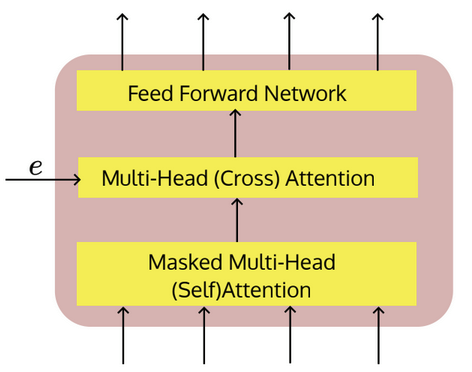
\includegraphics[width=\linewidth]{Degree//static/DL_decoder_block.png}
        \end{subfigure}
        \hfill
        \begin{subfigure}[b]{0.45\textwidth}
            \centering
            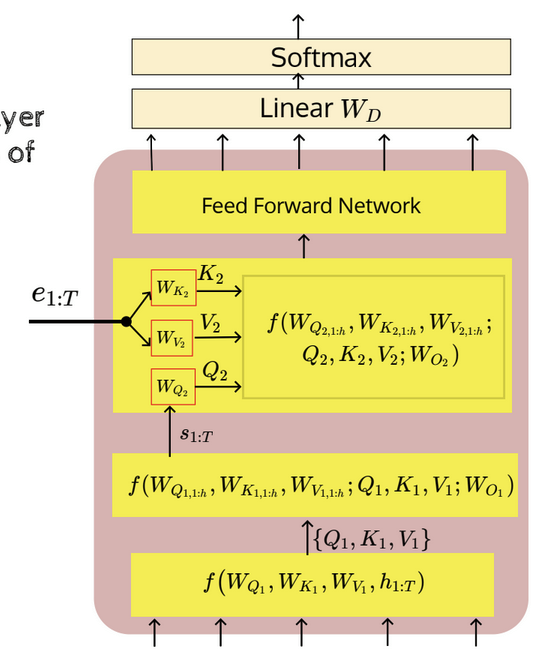
\includegraphics[width=\linewidth]{Degree//static/DL_decoder_block_detail.png}
        \end{subfigure}
        \caption{Decoder Block}
    \end{figure}
    \item We don't know how long is the output going to be, hence we will consider a max length $T_1$.
    \item At the beginning only $<GO>$ makes sense, all other inputs will be junk, hence we have "masked" self attention. Essentially, we make all $\alpha$ greater than current decoded word $0$.
    \item Masking is done by inserting negative infinite at the respective positions. This works because we take $\max$ of values(ReLU) in the feedforward network.
    \item We will also use masking in cross attention.
    \item We will take the values coming from encoder, and get $K$ and $V$. We will use output from self-attention as $Q$, then cross attention becomes the same as self-attention.
\end{itemize}

\end{document}